\documentclass[runningheads,a4paper]{llncs}
\usepackage{amssymb}
\usepackage{amsmath}
\usepackage{placeins}
\setcounter{tocdepth}{3}
\setlength\parindent{24pt}
\usepackage{graphicx}
\usepackage{textcomp}
\usepackage{epstopdf}
\usepackage{listings}
\usepackage{tabularx}
\usepackage{caption}
\usepackage{esvect}
\usepackage[skip=0pt]{caption}
\usepackage[margin=1 in]{geometry}
%\allowdisplaybreaks[1]
%\linespread{1.6}

\newenvironment{sciabstract}{%
\begin{quote} \bf}
{\end{quote}}

\usepackage{url}
\urldef{\mailsa}\path|fry2@case.edu|
\newcommand{\keywords}[1]{\par\addvspace\baselineskip
	\noindent\keywordname\enspace\ignorespaces#1}

\begin{document}

	\mainmatter  % start of an individual contribution
	% first the title is needed
	\title{Research Report}
	% a short form should be given in case it is too long for the running head
	\titlerunning{Young Research Report}
	\author{Fletcher Young}%
	%
	\authorrunning{Fletcher Young}
	% (feature abused for this document to repeat the title also on left hand pages)
	% the affiliations are given next; don't give your e-mail address
	% unless you accept that it will be published
	\institute{Case Western Reserve University\\
		Cleveland, OH 44106\\
		\mailsa\\}
	
	\maketitle
	\begin{sciabstract}
		This document is meant to serve as a documentation of research completed thus far.
	\end{sciabstract}
	
\section{Attachment Points}
	Muscle attachments in the first draft created for Living Machines were placed based on data from Johnson\textquotesingle s 2008 paper\cite{johnson_three-dimensional_2008}. In this paper, they list the xyz coordinates for every muscle attachment point on the rat hindlimb. This data is incredibly interesting and valuable for this project as it’s a biologically backed set of data for our model. The initial motivation for adhering to this data set was its experimental derivation. \par
			\begin{figure}
				\centering
				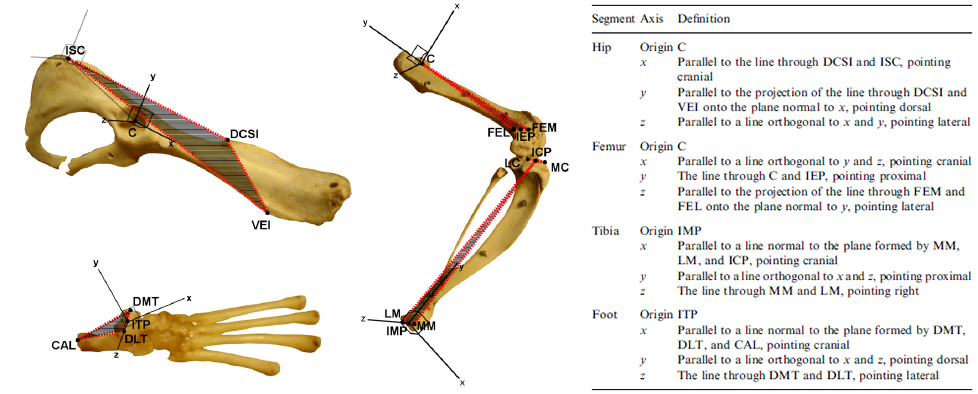
\includegraphics[width=\textwidth]{john1.PNG}
				\caption{The only demonstration of the bony-landmark-guided coordinate systems in Johnson's paper containing the muscle attachment points.}
			\end{figure}
	Johnson\textquotesingle s 2008 paper relates the muscle attachment coordinates in bone-centric coordinate systems defined by bony landmarks on the hind limb bones. While this is useful for generalization, there is no concrete placement of the these bony landmarks presented and the modeler is left approximating their positions based on a single figure from the paper. This leads to a large amount of potential error as changing the base coordinate system with skew the every attachment point in that coordinate system (sometimes as many as 24 attachment points). \par
			\begin{figure}
				\centering
				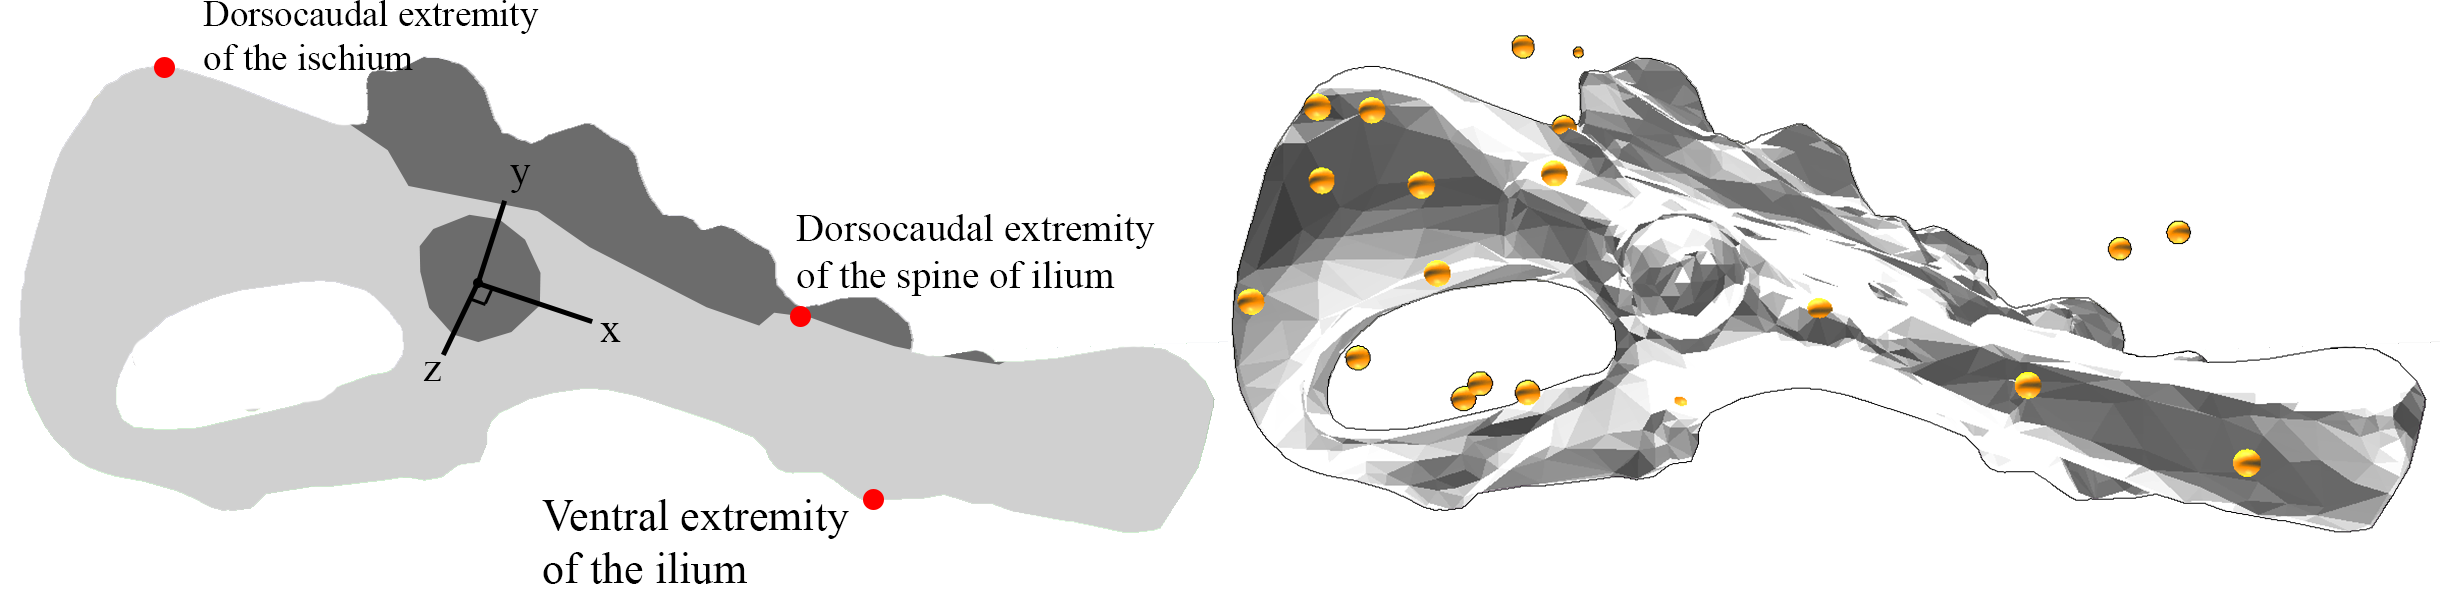
\includegraphics[width=\textwidth]{RP7.png}
				\caption{An example of utilizing Johnson's bony-landmark-based coordinate systems}
			\end{figure}
	Creative license had to be taken on some reference frames since attachments points were in anatomically impossible locations when using Johnson’s guidelines. The more we started to deviate away from the strict explanations of Johnson, the more personal creative enterprise we were taking and the less biologically representative the attachment coordinates became. There clearly needed to be a balance struck between applying new muscles in a way that made sense while also taking as much biological consideration as possible. \par
	The resulting model using Johnson’s coordinates was the one presented at Living Machines and demonstrates a much more complete hind limb model than what Alex finished with. This model has 38 muscles and around 80 muscle attachments. \par
			\begin{figure}
				\centering
				\begin{minipage}{0.5\textwidth}
					\centering
					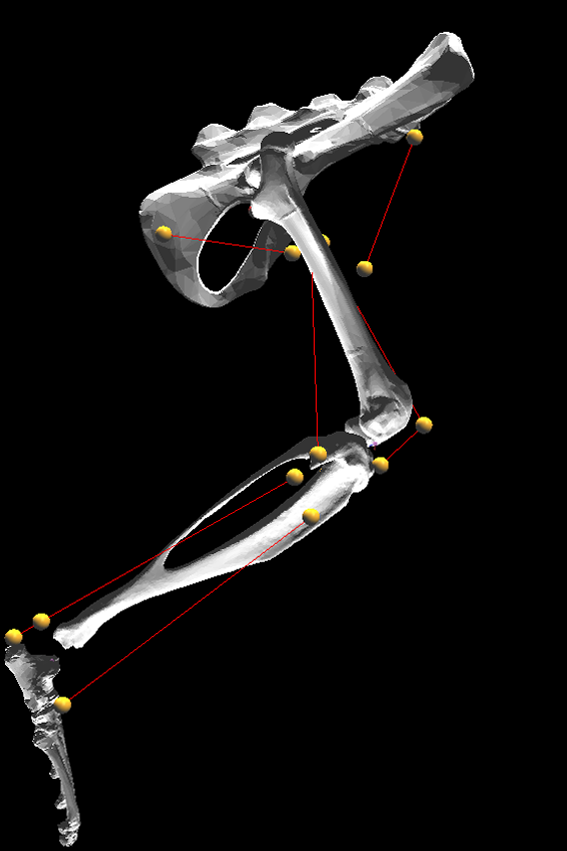
\includegraphics[width=\textwidth]{att2.PNG}
					\caption{Alex's leg model}
				\end{minipage}\hfill
				\begin{minipage}{0.5\textwidth}
					\centering
					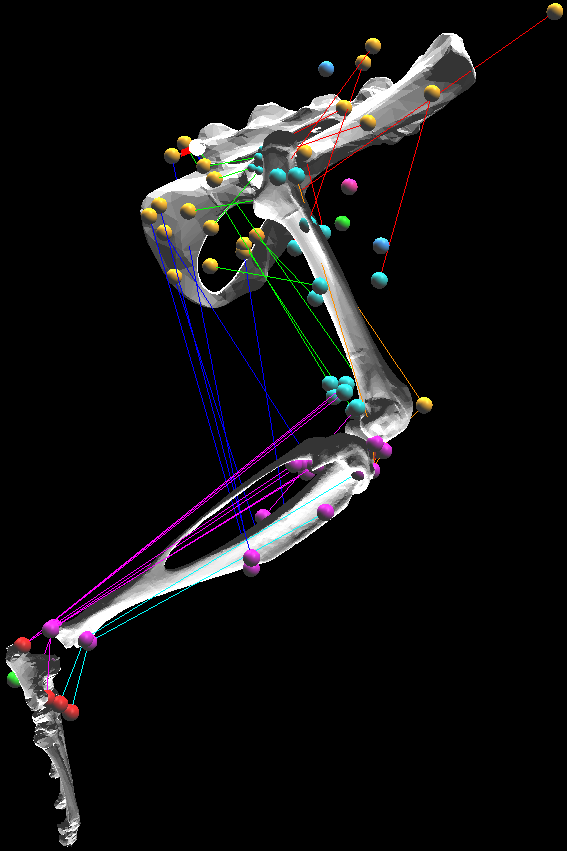
\includegraphics[width=\textwidth]{att1.PNG}
					\caption{First Draft of an Updated Model}
				\end{minipage}
			\end{figure}
	After returning from Living Machines and consulting with Alex and Christian Rode (a lab member of our partner institution in Jena, Germany), it became clear that the model would not be useful in its current form. This was mainly due to the fact that many muscles actually passed through bones when the joints were moved through their range of motion. For example, the biceps femoris anterior, whose origin is on the spine, would pass through the pelvis when connecting to its insertion inside the knee. \par
			\begin{figure}
				\centering
				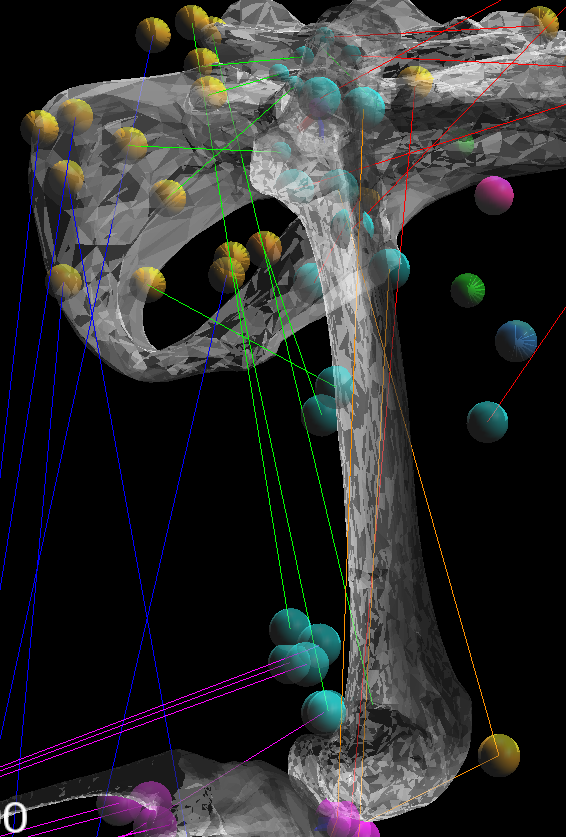
\includegraphics[width=.5\textwidth]{att8.PNG}
				\caption{Semi-transparent bones reveal muscle paths passing through bone. Notably, the vastus muscles (orange) passing through the femur and inserting onto the tibia.}
			\end{figure}
	At this point, we turned to the literature and found an anatomical primer on the rat: Eunice Chase Greene\textquotesingle s 1935 \underline{Anatomy of the Rat}\cite{greene_anatomy_1955}. This resource is a goldmine for anatomical drawings and images of the rat. Every biological system (muscular, nervous, circulatory, etc.) is highly detailed. \par
	Using Greene\textquotesingle s book, we analyzed every muscle individually to try to match its muscle path from origin to insertion. Via points were added to simulate muscle wrapping around bones. In this case, the biceps femoris anterior now would pass over the dorsocaudal ridge of the ischium and insert into the tendinous sheath at the distal end of the femur. \par
	viii.	The resulting model based on Greene’s work much more closely aligns with the anatomical representation of the rat hind limb. Muscles no longer pass through bones at any point during the walking cycle. \par
			\begin{figure}
				\centering
				\begin{minipage}{0.5\textwidth}
					\centering
					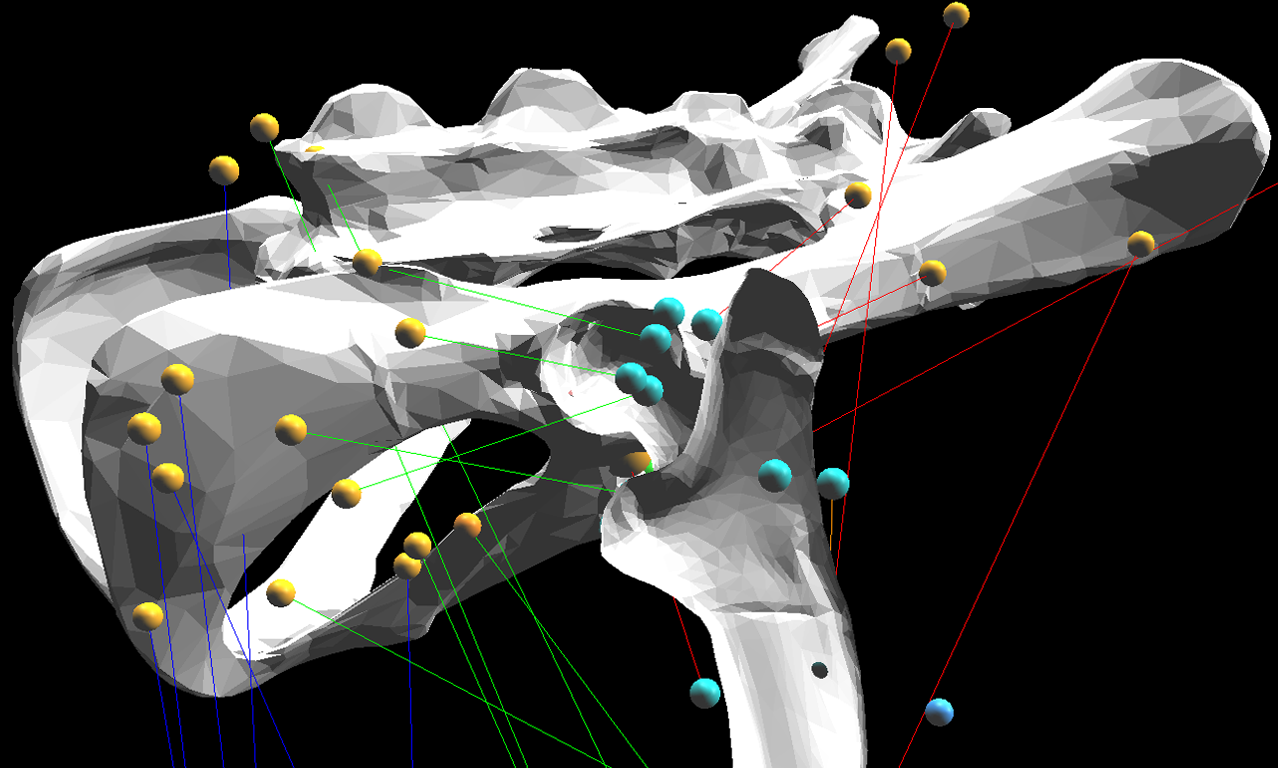
\includegraphics[width=\textwidth]{pel1.PNG}
					\caption{Model using Johnson's coordinates}
				\end{minipage}\hfill
				\begin{minipage}{0.5\textwidth}
					\centering
					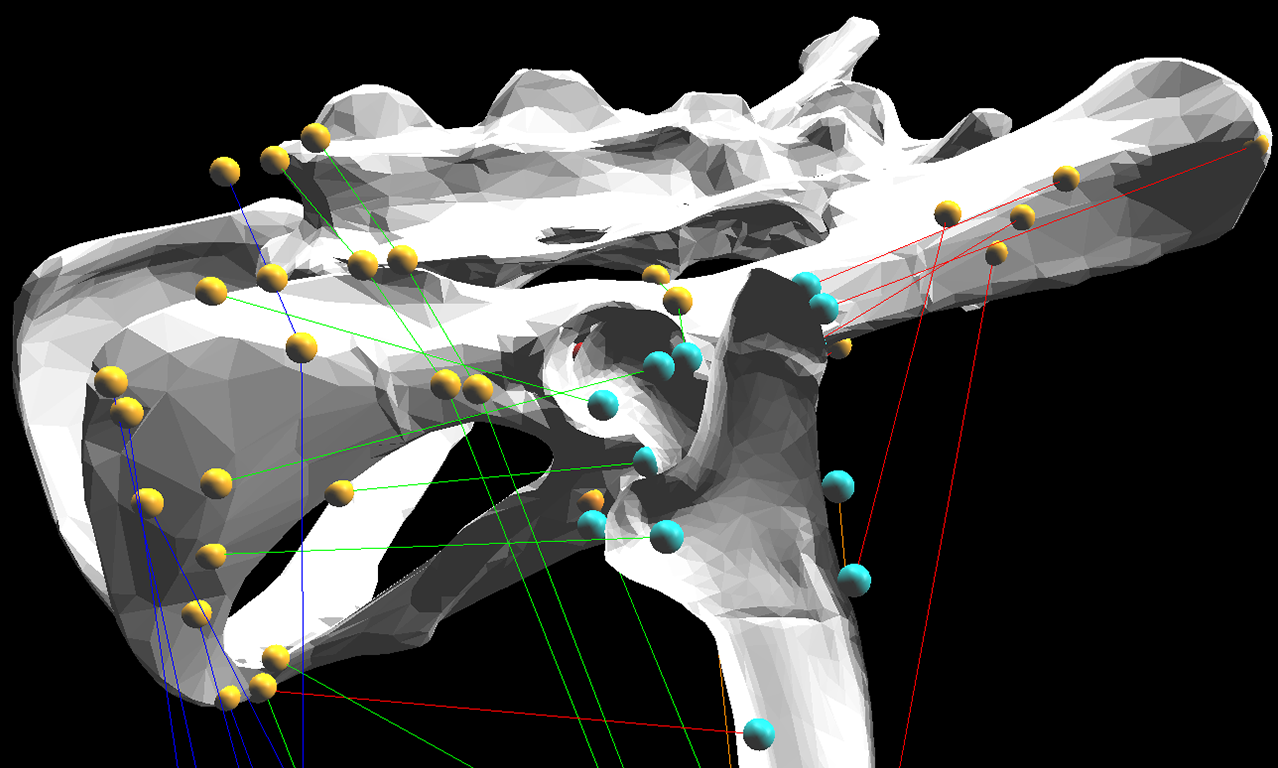
\includegraphics[width=\textwidth]{pel2.PNG}
					\caption{Model using Greene's explanations and figures}
				\end{minipage}
			\end{figure}
	Two areas of note regarding the revised model are at the knee and ankle. Animatlab does not represent muscle wrapping and is only able to simulate muscle attachment points stationary within bone coordinate systems. For this reason, knee and ankle extensors were moved away from the bones surfaces in order to simulate the fulcrum motion of those muscles. In particular, the vastus muscles of the knee loop over the end of the femur and insert into a common point representing the tuberosity of the tibia. Similarly, ankle extensors insert into a simulated Achilles tendon in order to prevent bone pass-through. \par
			\begin{figure}
				\centering
				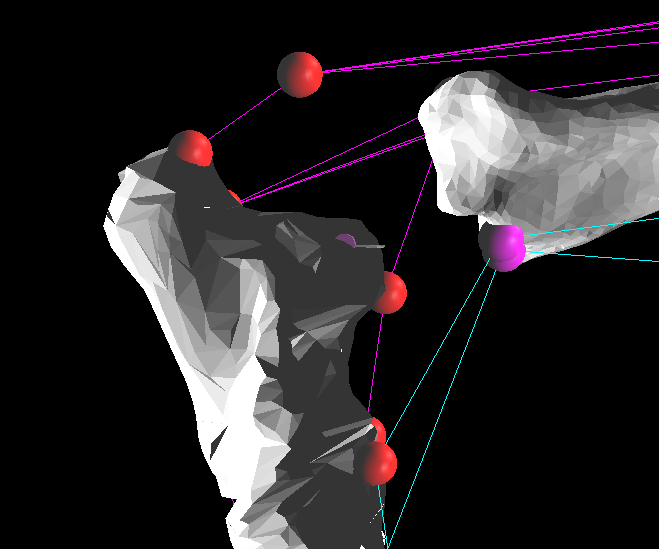
\includegraphics[width=.5\textwidth]{att4.PNG}
				\caption{Revised ankle joint with a moving Achilles tendon}
			\end{figure}
			\begin{figure}
				\centering
				\begin{minipage}{0.6\textwidth}
					\centering
				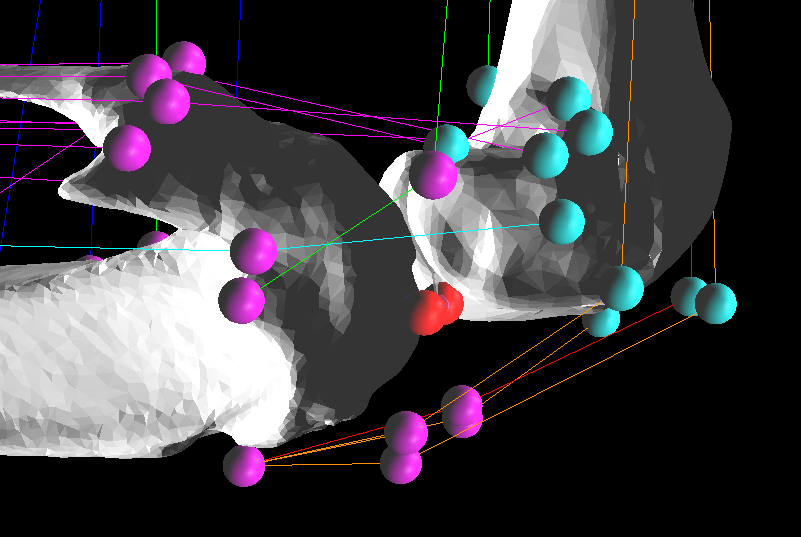
\includegraphics[width=\textwidth]{att5.PNG}
				\caption{Revised knee joint without bone pass through}
				\end{minipage}\hfill
				\begin{minipage}{0.4\textwidth}
					\centering
					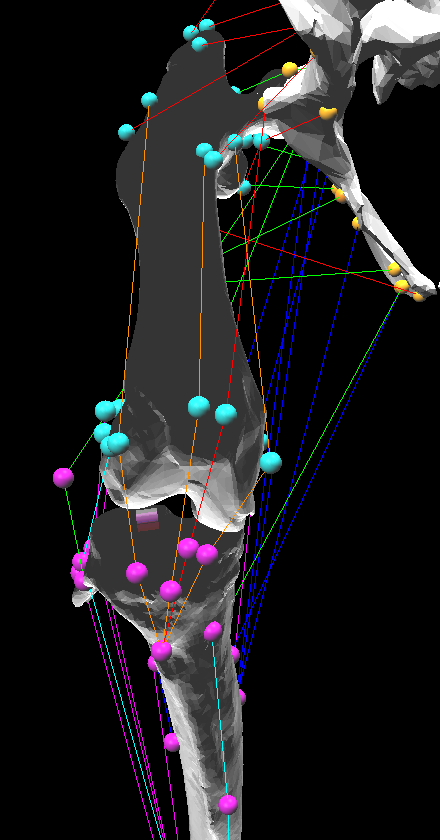
\includegraphics[width=\textwidth]{att6.PNG}
					\caption{Front of the knee}
				\end{minipage}
			\end{figure}
			\FloatBarrier
	These approximations are not perfect but in a simulation environment without muscle wrapping or moving attachment points, they are just about the best we can do. There is still plenty of information and research that can be conducted with them. \par
			\begin{figure}
				\centering
				\begin{minipage}{0.5\textwidth}
					\centering
					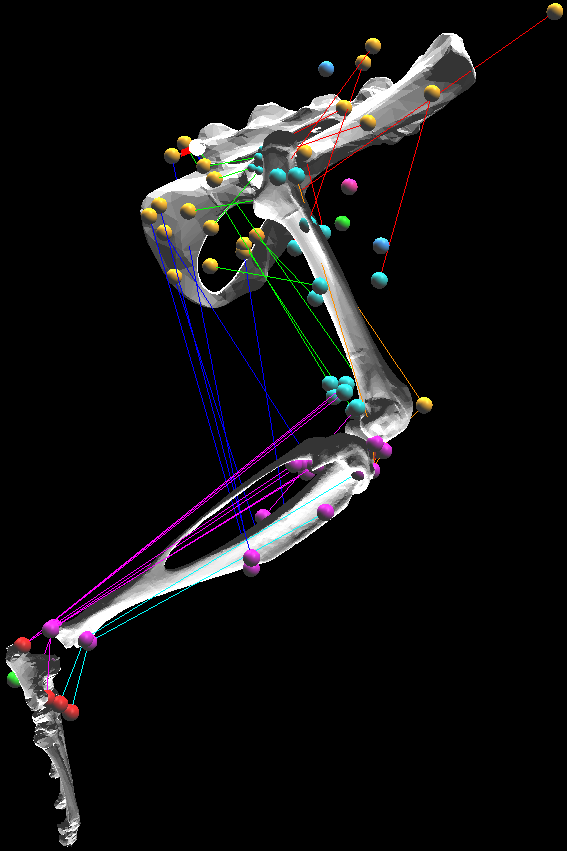
\includegraphics[width=\textwidth]{att1.PNG}
					\caption{Model based on Johnson's coordinates}
				\end{minipage}\hfill
				\begin{minipage}{0.5\textwidth}
					\centering
					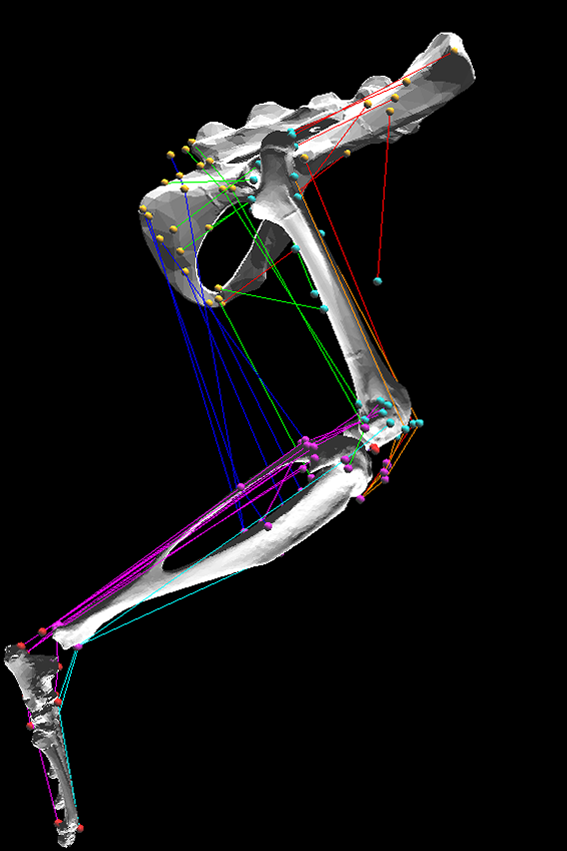
\includegraphics[width=\textwidth]{att3.PNG}
					\caption{Current model based on Greene's book}
				\end{minipage}
			\end{figure}
			
	\section{Accurate Joint Limits}
	I wanted to generate a realistic walking signal in Animatlab by driving the joints in a biologically representative way. In order to drive the joint angles correctly, I needed to first confirm the joint ranges were appropriate. Examining the existing joint ranges, I found that they did not match work previously found by Martin Fischer, the head of our collaborative lab in Jena, Germany. I decided to rework the joints to fit his data\cite{fischer_basic_2002}. \par
	I analyzed the joint ranges for each phase of gait (touch down, lift off, etc) and found the absolute maximum and minimum positions for each joint. I used these as my joint bounds. \par
			\begin{figure}
				\centering
				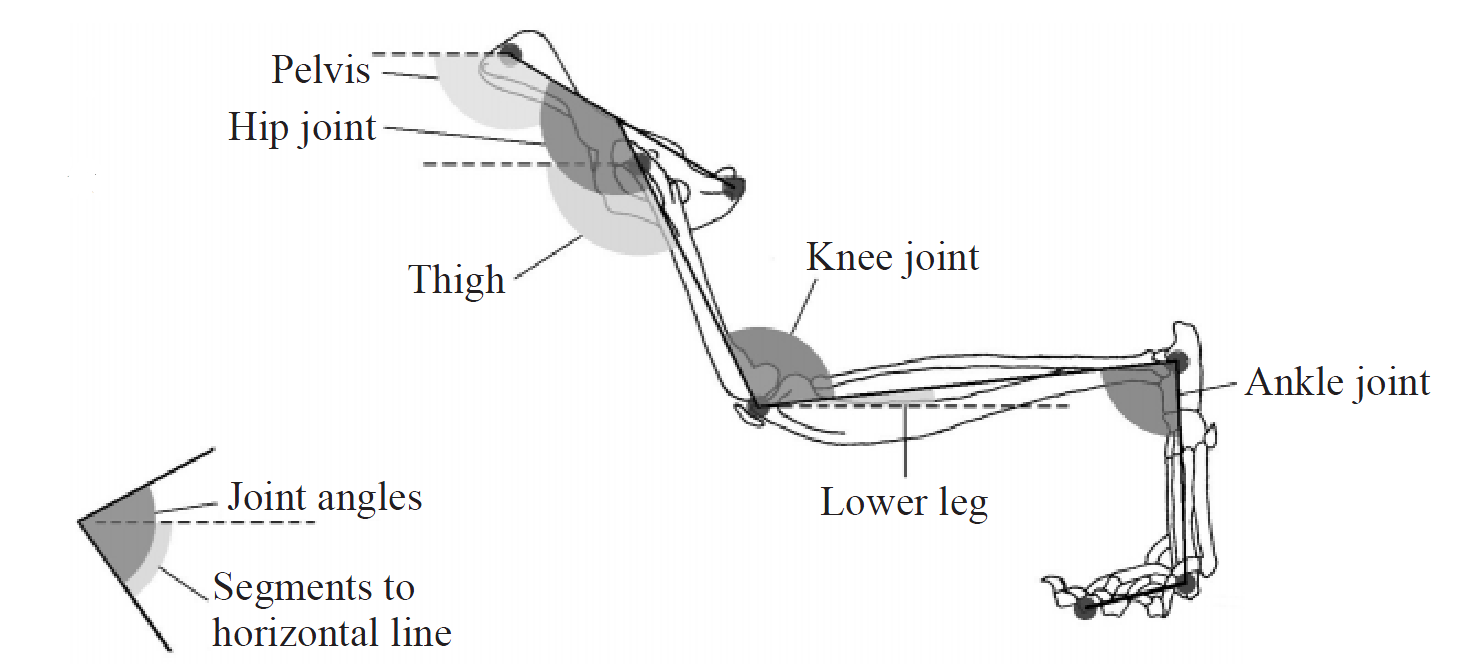
\includegraphics[width=.8\textwidth]{FischerAngles4.PNG}
				\caption{Joint angle scheme for Dr. Fischers 2002 paper}
			\end{figure}
			\begin{figure}
				\centering
				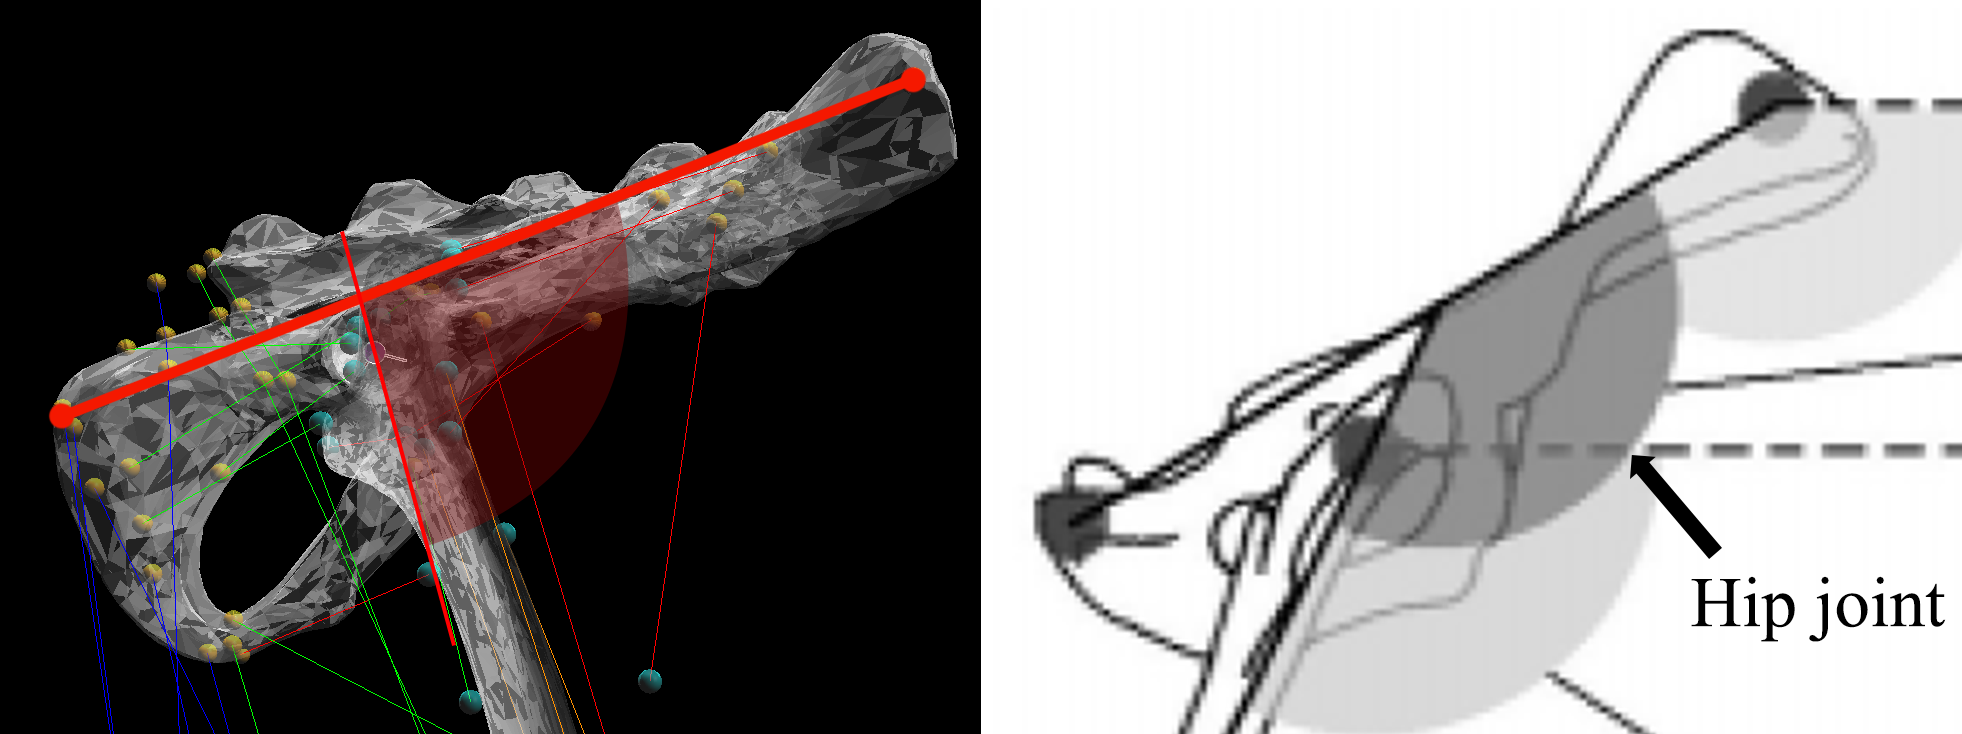
\includegraphics[width=\textwidth]{FischerAngles2.png}
				\caption{Comparing the simulation model with the model in the paper}
			\end{figure}
	Fischer provided gait profiles for the hip, knee, and ankle for a single step. Fischer included a compilation image of different animals’ gait patterns. I used Photoshop to extract the gait profile for the \textit{Rattus norvegicus}. In Photoshop, I mapped pixel lengths to joint angles. This gave me a collection of joint angles during the stride length from which I was able to construct a position waveform in Animatlab. \par
			\begin{figure}
				\centering
				\begin{minipage}{0.5\textwidth}
					\centering
					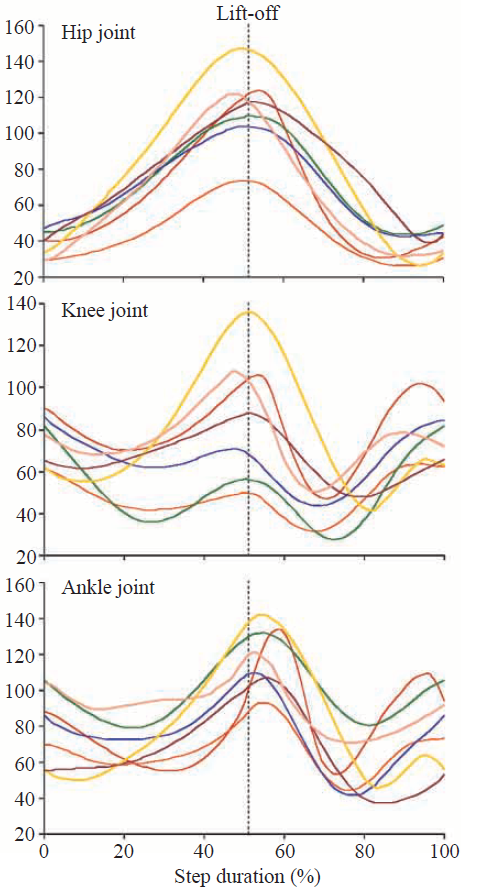
\includegraphics[width=\textwidth]{FischerAngles.PNG}
					\caption{Full gait profiles for all of the organisms}
				\end{minipage}\hfill
				\begin{minipage}{0.5\textwidth}
					\centering
					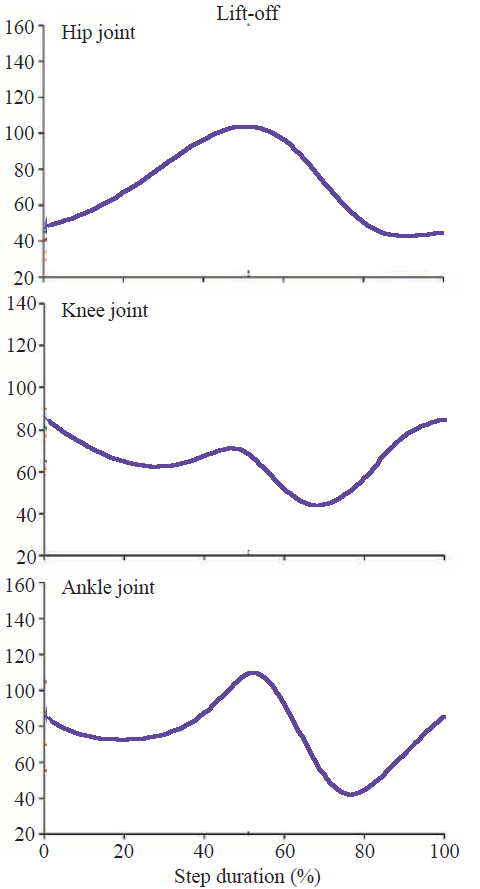
\includegraphics[width=\textwidth]{FischerAngles3.png}
					\caption{Isolated gait profile of the \textit{Rattus norvegicus}}
				\end{minipage}
			\end{figure}
	To do this, I used the curve fit tool in Matlab, creating a sum of sines waveform that I could copy into Animatlab. \par
	A few weeks after generating these waveforms, Alex sent in data regarding his torque calculations. Within this code were his simulations of joint angles. Based on data from our Jena collaborators, Alex was able to directly transcribe the stance phase joint angles. In order to supplement the missing swing phase joint angles, he simulated the rat hindlimb in Simulink and fit the data for a complete cycle. \par
			\begin{figure}
				\centering
				\begin{minipage}{0.5\textwidth}
					\centering
					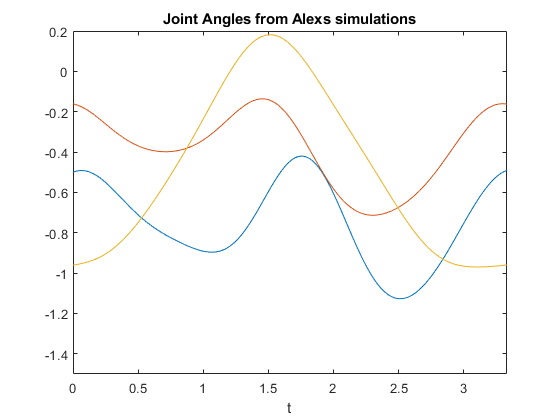
\includegraphics[width=\textwidth]{jointangles3.png}
					\caption{Full gait profiles for all of the organisms}
				\end{minipage}\hfill
				\begin{minipage}{0.5\textwidth}
					\centering
					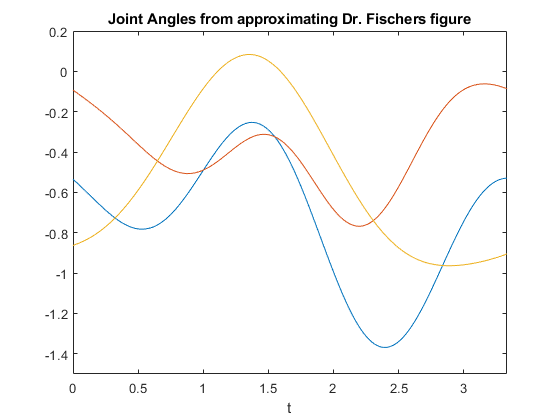
\includegraphics[width=\textwidth]{jointangles4.png}
					\caption{Isolated gait profile of the Rattus norvegicus}
				\end{minipage}
			\end{figure}
	The waveforms generated from Dr. Fischer\textquotesingle s figure and Alex\textquotesingle s simulations are very similar. Due to the concrete, data-driven method Alex devised, I decided to implement his waveforms into Animatlab. It’s possible in the future that we can analyze key performance outcomes for both waveforms and decide which one is more accurate. \par
	
	\section{Muscle Length and Velocity}
	To calculate muscle lengths in Matlab, we export the simulation file from Animatlab. This simulation file is simply a text document containing all objects and properties related to the simulation. By scraping the text document for specific key words, we are able to convert any simulation document into an object hierarchy within Matlab. \par
	Within the Matlab code, each leg of the animal (currently just the left hindlimb) is represented as an object that contains three joint objects and thirty eight muscle objects. These “objects” act as distinct entities within the code, holding parameter values and pieces of information relevant to that specific object (e.g. muscle damping is stored in the muscle). This keeps code organized as there are dozens of attachments, muscles, and thousands of distinct timesteps. \par
	The initial muscle attachment points are scraped from Animatlab and stored in the muscle objects. These points include the origin, insertion, and all via points. There is no limit to the number of via points that can be used on a muscle, allowing us to loop muscles over and around bones. These attachment points are stationary within the local bone frames, though, so we are unable to model muscle slipping over the surface of bones or contact with other muscles. \par
			\begin{figure}
				\centering
				\begin{minipage}{0.48\textwidth}
					\centering
					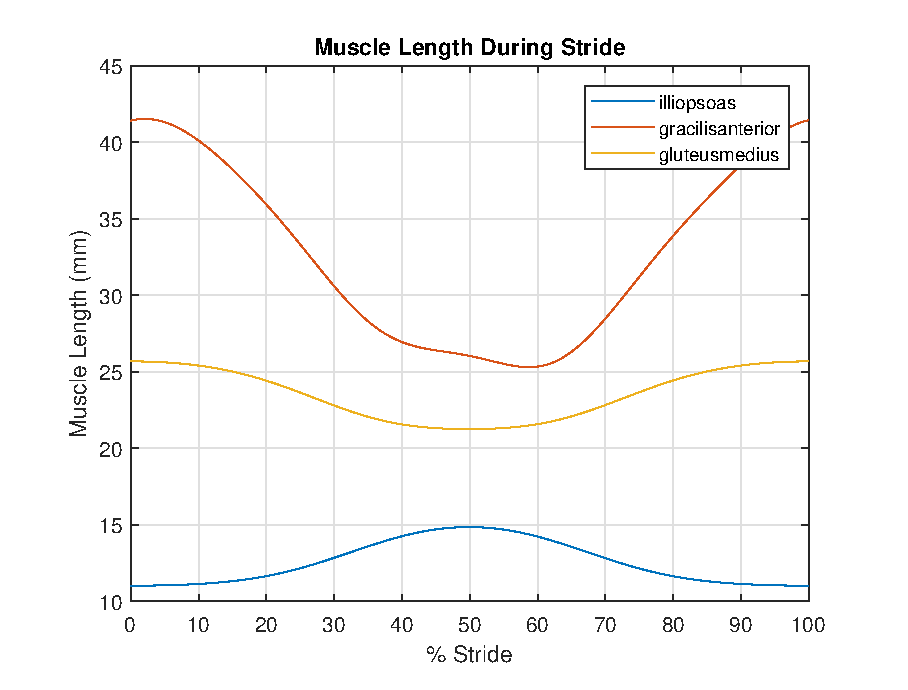
\includegraphics[width=\textwidth]{musc2.eps}
					\caption{Muscle Length Calculated in Matlab using the principles of local reference frames}
				\end{minipage}\hfill
				\begin{minipage}{0.48\textwidth}
					\centering
					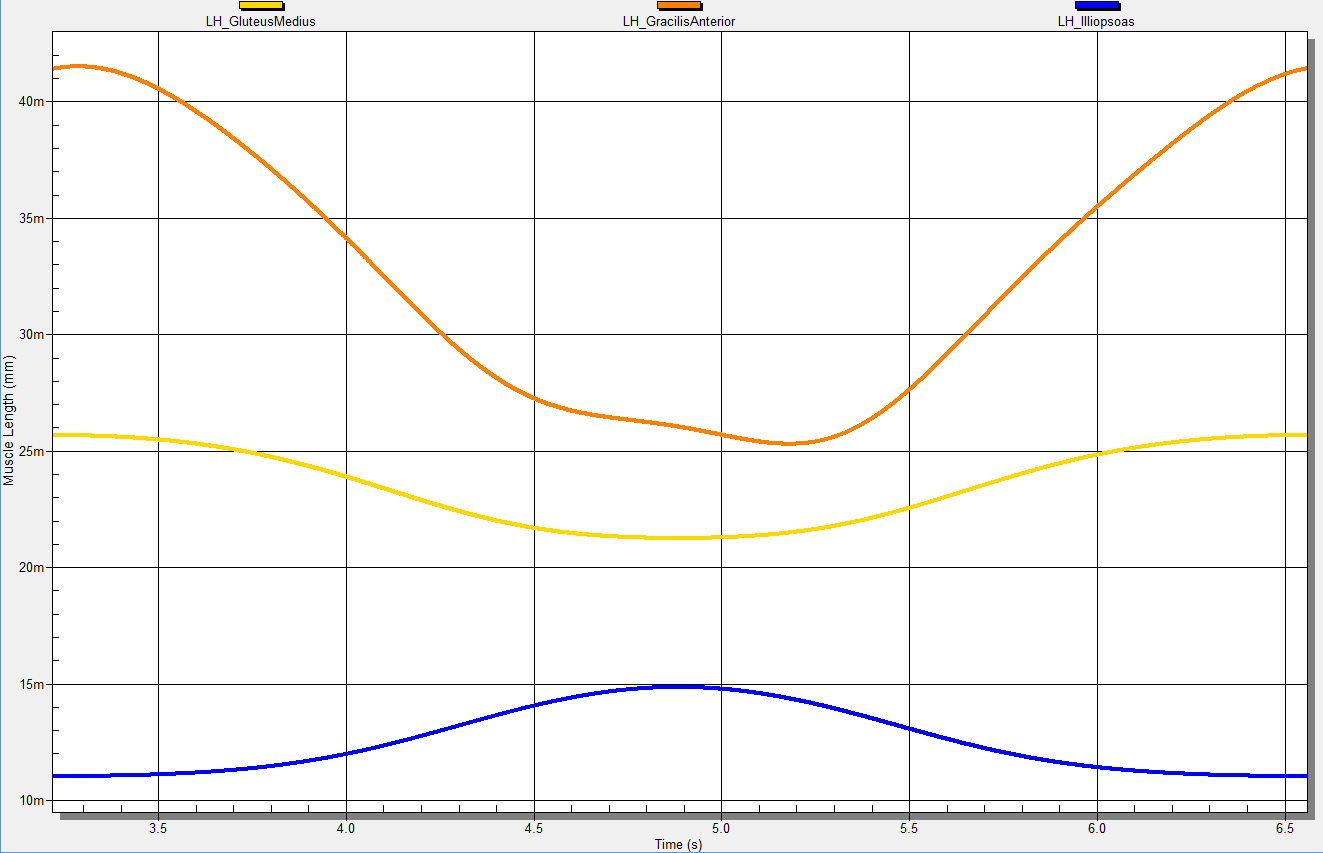
\includegraphics[width=\textwidth]{musc3.PNG}
					\caption{Muscle Length simulated in Animatlab. Currently the "gold standard" metric for which to compare Matlab code results}
				\end{minipage}
			\end{figure}
	Attachment points are then moved through the walking motion dictated by the chosen walking pattern. As mentioned previously, this is the joint angle profile that Alex simulated. At each distinct timepoint (once every .0005 seconds), every muscle attachment position is calculated. From these attachment positions, it’s possible to develop a muscle length profile over the gait cycle. \par
	From this information, every muscle object contains the extreme lengths reached (L{\scriptsize min},L{\scriptsize max}), the muscle length profile, and the muscle velocity profile. These pieces of information are extremely useful in determining muscle and joint parameters. \par
	
	\section{Analysis of Muscle Parameters}
	The analysis of muscle parameters is a delicate art, as muscle properties are distinct from animal to animal and from experiment to experiment. This work strives to form as complete a picture as possible of the muscle properties for the rat hindlimb and connects a number of different sources on the best approach to supplement these  parameters where they do not exist directly in the literature. As each of these parameters have their own distinct calculations and explanations, I've broken them up into separate subsections.
	\subsection{Johnson's 2001 Parameters}
	Will Johnson out of Dr Edgerton's lab at UCLA put out a paper in 2011 titled "Application of Rat Hindlimb Model: A Prediction of Force Spaces Reachable Through Stimulation of Nerve Fascicles".\cite{johnson_application_2011} This work contains experimental muscle parameters for each muscle in the rat hindlimb. 
	\begin{quote}
	 "...architectural measurements including mass, optimal fiber length, maximum isometric tension and maximum shortening velocity were taken from n=4 rats, while electrophysiological measurements of maximum isometric tension and shortening velocity, and tendon slack lengths were taken from n=2 rats."
	\end{quote} \par
	\subsection{Eng's 2008 Parameters}
	Carolyn Eng of Dr. Richard Lieber's lab at the Departments of Orthopaedic Surgery and Bioengineering, University of California and Veterans Administration Medical Centers put out a paper in 2008 titled "Scaling of muscle architecture and fiber types in the rat hindlimb". This paper contains hindlimb muscle data akin to Johnson's with the addition of the physiological cross sectional area (PCSA) and the fiber length percentage (Lf/Lm). \par
	Since Johnson's previous work had motivated the naming conventions of muscles during the attachments phase, I chose to use his data primarily for the muscles in the model. However, almost all of Johnsons work is for muscle fibers, which needed to be expanded for the full muscles. For this, I use Eng's fiber length percentages to convert Vmax fiber to Vmax muscle.
	\subsection{The Hill Muscle Model}
			\begin{figure}
				\centering
				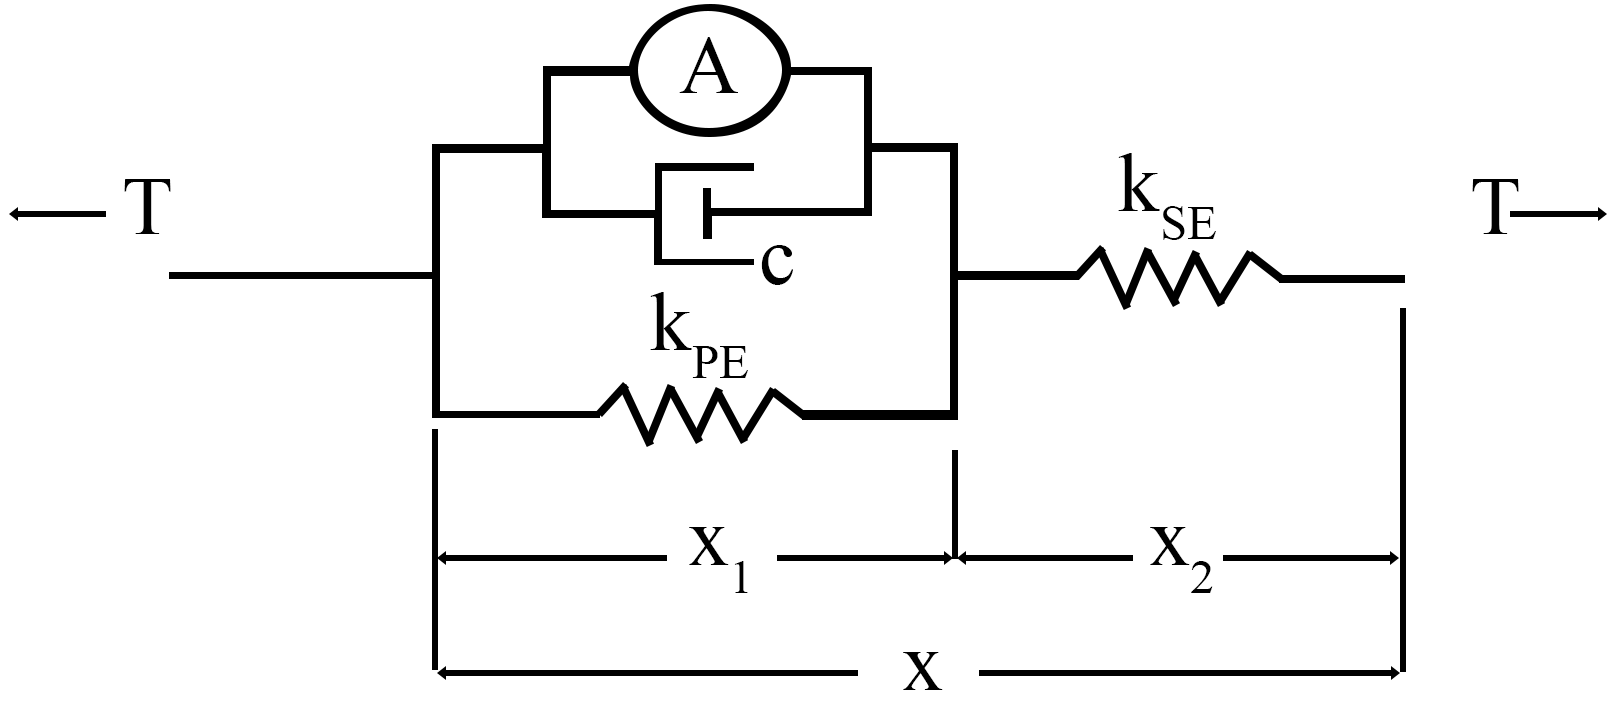
\includegraphics[width=.7\textwidth]{hill1.png}
				\caption{The Linear Hill Muscle Model}
				\label{fig:hill}
			\end{figure}
		A review of Animatlab's muscle model if important to understand the relevance of the various muscle parameters that must be calculated. Animatlab utilizes a linear Hill muscle model. This model, shown in Fig. \ref{fig:hill}, represents the viscoelastic qualities of muscle. A complete rat hindlimb model must include active and passive parameters for every muscle in the hindlimb. At this point, that amounts to parameters for thirty eight muscles, most of which are not explicitly outlined in the literature. This means that we must make approximations of the parameters based on the information we have.
	\subsection{Kse}
		The series elastic element (Kse) represents the tendon stiffness of the muscle. The greatest resource in addressing muscle parameters has been Felix Zajac's 1989 paper titled "Muscle and Tendon: Properties, Models, Scaling, and Application to Biomechanics and Motor Control"\cite{zajac_muscle_1989}. In this work, Zajac suggests using a generic force-strain curve to determine tendon stiffness. Johnson's paper lists the tendon slack length for multiple muscles and the maximum force of each muscle, allowing us to calculate the series elastic element for each muscle.
			\begin{figure}
				\centering
				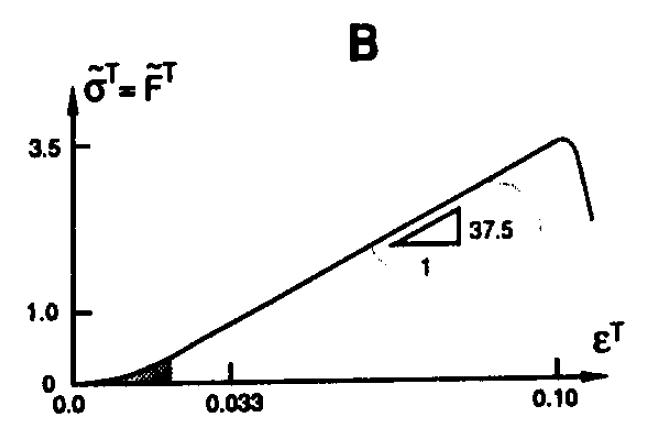
\includegraphics[width=.5\textwidth]{zajac1.PNG}
				\caption{Zajac's generic force-strain curve for muscle tendon}
				\label{fig:zajac1}
			\end{figure}
		Zajac's curve relates the normalized tendon strain to the normalized tendon stress, which in this case equals the normalized muscle tension. Normalized tendon stress equals normalized tendon force under the assumption that the optimal tendon stress is 32MPa:
			\begin{align*}
				\tilde{\sigma}^{T} &= \frac{\sigma^{T}}{\sigma_{o}^{T}}
				= \frac{\sigma^{T}}{\frac{F_{o}^{M}}{A^{T}}}
				= \frac{\frac{F^{T}}{A^{T}}}{\frac{F_{o}^{M}}{A^{T}}}
				= \frac{F^{T}}{F_{o}^{M}}
				= \tilde{F}^{T}
			\end{align*}
		where $\tilde{\sigma}^{T}$ is the normalized tendon stress, $\sigma_{o}^{T}$ is the optimal tendon stress, $F_{o}^{M}$ is the optimal muscle tension, $A^{T}$ is the tendon cross sectional area, and $\tilde{F}^{T}$ is the normalized tendon force. \par
		Tendon strain is determined based on the assumption that the nominal tendon strain is 3.3\%:
			\begin{align*}
				\epsilon^{T} &= \frac{\Delta L^{T}}{L_{s}^{T}}
				= \frac{L^{T}-L_{s}^{T}}{L_{s}^{T}}
				= \frac{L^{T}}{L_{s}^{T}} - 1 \\
				K_{se} &= \frac{\Delta F}{\Delta L}
				= \frac{\Delta F}{(\Delta \epsilon+1)L_{s}^{T}}
				= \frac{3.5 F_{o}^{M} - F_{o}^{M}}{1.1 L_{s}^{T} - 1.033 L_{s}^{T}}
				= 37.5 \frac{F_{o}^{M}}{L_{s}^{T}}
			\end{align*}
		where $\epsilon^{T}$ is the normalized tendon strain, $L^{T}$ is the tendon length, and $L_{s}^{T}$ is the tendon slack length. With this generalized curve, it's possible to calculate serial elastic parameters for all muscles using their maximum force and tendon slack length. This works well for those muscles in Johnson's paper that have measured tendon slack lengths. Some of the muscles do not have recorded tendon slack lengths, though. For these muscles I checked the Kse values against existing muscle parameters and found a trend between the muscle's mass and Kse.
			\begin{figure}
				\centering
				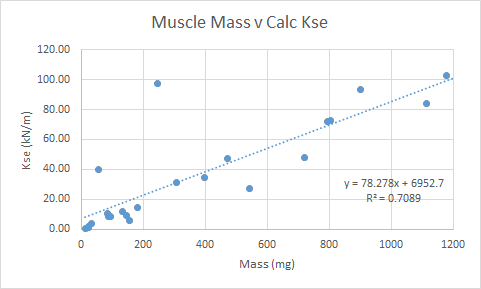
\includegraphics[width=.7\textwidth]{zajac3.png}
				\caption{Correlation between mass and Kse for those muscles with a measured tendon slack length}
				\label{fig:zajac3}
			\end{figure}
		While not a perfect metric, this allows us to make some approximation for the tendon slack lengths we're missing and to generate serial elastic values for each muscle.
		
	\subsection{Kpe}
		The parallel elastic element can be calculated if we assume that the series and parallel elastic elements absorb all tension when the muscle is at a set length. By this assumption, we can treat the muscle as a simple two-spring system under load. Assuming the muscle exerts 70\% of their maximum force when fully contracted and knowing the values of Kse, we can find Kpe.
			\begin{align*}
				F &= K_{eq} x \\
				\Delta F &= K_{eq} \Delta L \\
				(F_{max} - .7 F_{max}) &= K_{eq} (L_{max}-L_{min}) \\
				.3 F_{max} &= \frac{K_{se}K_{pe}}{K_{se}+K_{pe}} (L_{max}-L_{min}) \\
				K_{pe} &= \frac{.3 F_{max} K_{se}}{K_{se} (L_{max}-L_{min})- .3 F_{max}}
			\end{align*}
		where $F_{max}$ is supplied by Johnson's 2011 paper, Kse is calculated as previously discussed, and the length limits determined by computing the muscle length profiles.
	\subsection{Damping}
	\begin{align*}
		c &= \frac{F_{max}}{v_{f}^{M}*\big(\frac{L_{f}}{L_{m}}\big)} \\
		c &= \frac{F_{max}}{v_{max}} \\
	\end{align*}
	\subsection{Lwidth}
			\begin{figure}
				\centering
				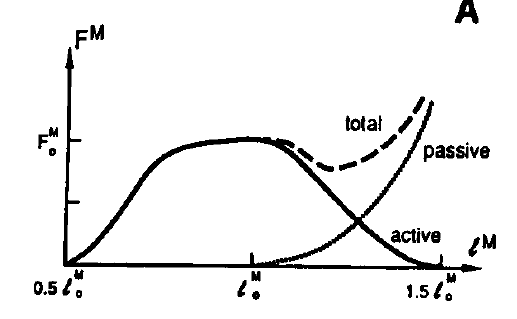
\includegraphics[width=.7\textwidth]{lwidth3.PNG}
				\caption{Nominal length-tension curve for muscle}
				\label{fig:lwidth3}
			\end{figure}
		The length-tension (LT) curve of muscle is used to map the length of the muscle to its ability to produce force. Zajac presents a general form of a muscle's LT curve in Fig. \ref{fig:lwidth3}. At an optimal length that's different for every muscle, that muscle is able to produce the most isometric force. Below this optimal length, the muscle's ability to produce force is diminished. As the muscle is pulled to a supraoptimal length, passive forces within the muscle begin to accumulate, enhancing the muscle's ability to generate tension simply due to its structure. \par
				\begin{figure}
					\centering
					\begin{minipage}{0.68\textwidth}
						\centering
						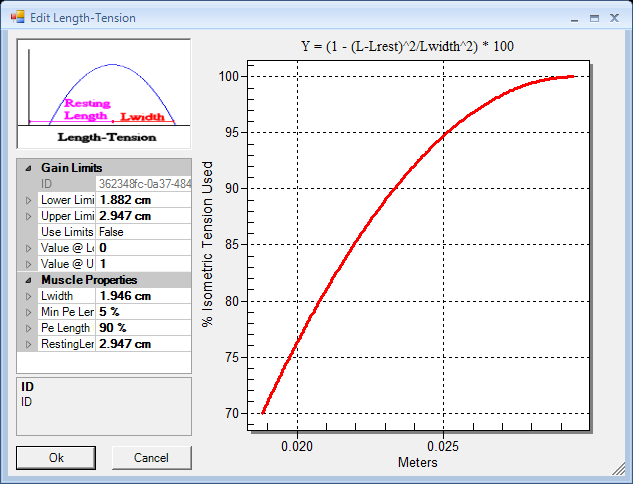
\includegraphics[width=\textwidth]{lwidth5.PNG}
						\caption{Animatlab's length tension curve}
						\label{fig:animatlabLT}
					\end{minipage}\hfill
					\begin{minipage}{0.28\textwidth}
						\centering
						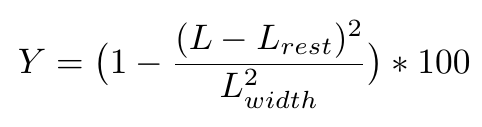
\includegraphics[width=\textwidth]{lwidth2.PNG}
						\caption{Equation used to calculate the muscle tension curve}
					\end{minipage}
				\end{figure}
		Animatlab presents a simplified version of the LT curve, shown in Fig. \ref{fig:animatlabLT}. The muscle width is a property that Animatlab uses to define its simplified length-tension curve. Prior work by Christian Rode on the cat soleus shows an experimentally derived LT curve, shown in Fig. \ref{fig:christianLT}. This curve maps normalized force against muscle deviation from its optimal length. In this case, a length of zero on the abscissa represents the muscle at its optimal length. As reported by Christian, the optimal length "the optimal length is about 10\% longer than in classically determined [force length relationships]". \par
				\begin{figure}
					\centering
					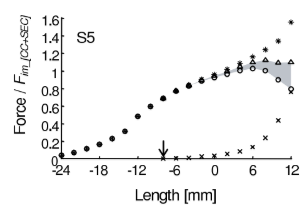
\includegraphics[width=.7\textwidth]{lwidth4.PNG}
					\caption{Christians LT curve}
					\label{fig:christianLT}
				\end{figure}
		In Fig. \ref{fig:christianLT}, the resting length is represented by an arrow. The corresponding force at this point is about 70\% of the maximum force, implying that the Animatlab simplification by use incorrect terminology when representing the resting length. Fig. \ref{fig:LTcompare} highlights the discrepancy. Functionally, this isn't much of an issue as long as it's acknowledged that the resting length entered into Animatlab is actually the optimal muscle length.
				\begin{figure}
					\centering
					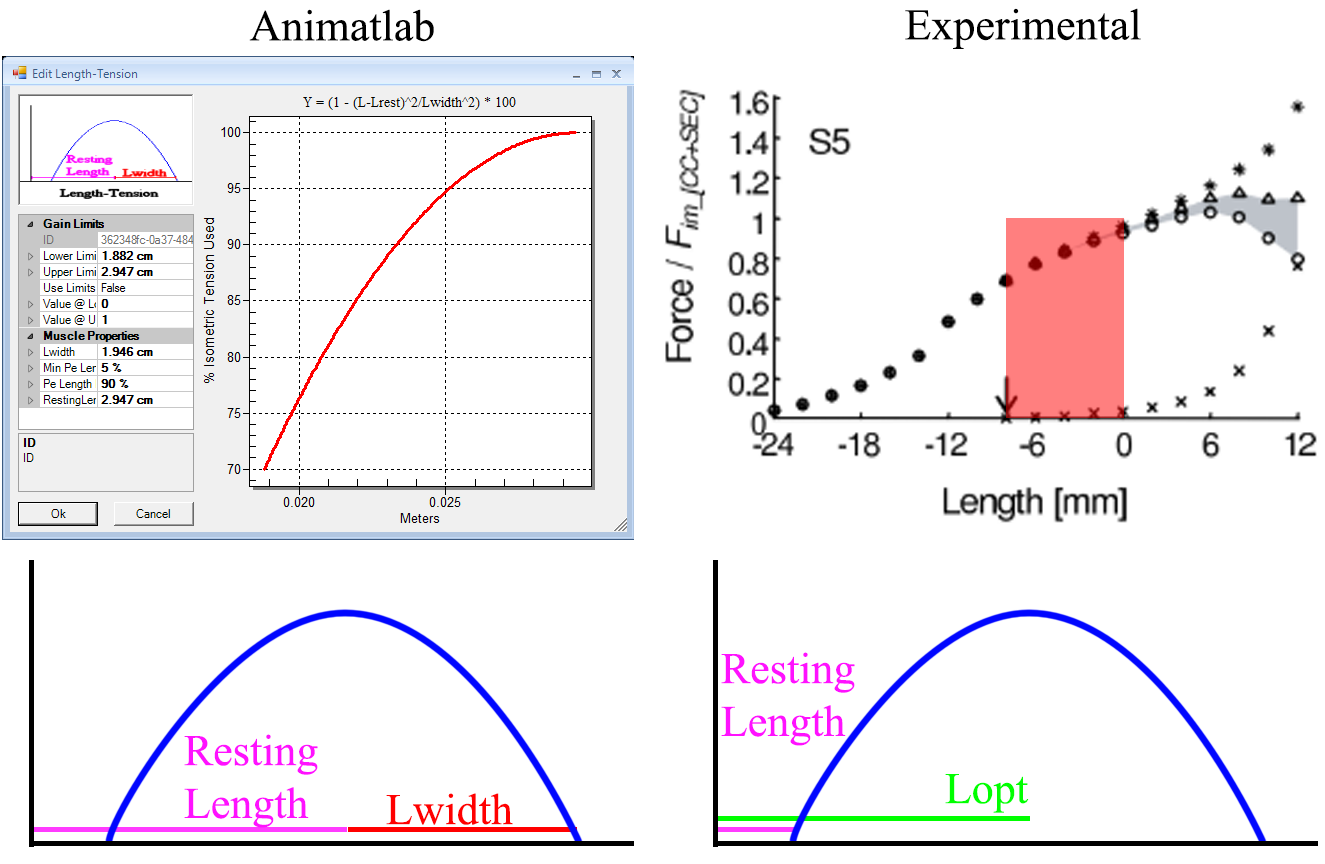
\includegraphics[width=.7\textwidth]{lwidth6.png}
					\caption{A comparison of Animatlab's LT terminology and experimentally derived terminology}
					\label{fig:LTcompare}
				\end{figure}
		Christian's work shows that the passive tension begins to manifest once the muscle is stretched beyond its resting length. The previous model is predicated on the assumption that all muscle activity operates within the ascending limb of the LT curve, where the muscle only becomes stronger as it is elongated to its maximum length. This means that for a given walking profile (which determines the muscle length profile), every muscle is capable of generating 70\% of its maximum tension at its minimum length and 100\% of its maximum tension at its maximum length.
		Based on these assumptions and Animatlab's LT simplification formula, $L_{width}$ can be calculated for each muscle:
			\begin{align*}
				Y &= \big(1-\frac{(L-L_{rest})^2}{L_{width}^2}\big)*100 \\
				.3 &= \frac{(L-L_{rest})^2}{L_{width}^2} \\
				L_{width} &= \frac{|L-L_{rest}|}{\sqrt{.3}} \\
			 L_{width} &= \frac{|L_{min}-L_{max}|}{\sqrt{.3}}
			\end{align*}
	\subsection{Stimulation-Tension Curve}
			\begin{figure}
				\centering
				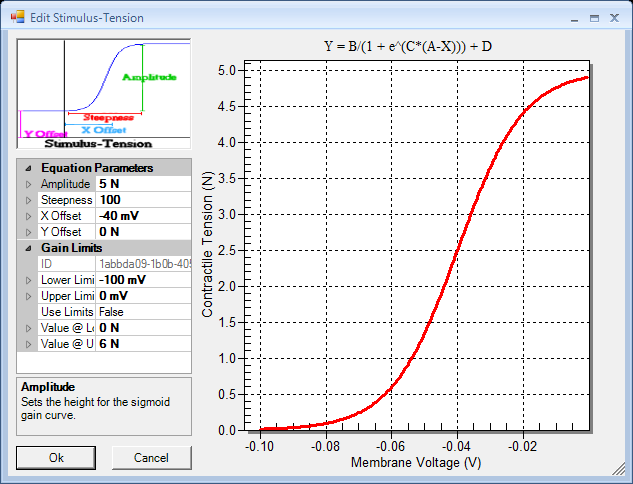
\includegraphics[width=.8\textwidth]{st2.PNG}
				\caption{A stimulus-tension curve in Animatlab}
				\label{fig:STanim}
			\end{figure}
		While most work hasn't utilized this curve yet because I haven't included muscle activations, it is important to include the parameters related to the stimulus tension (ST) curve. This curve relates the membrane voltage of the motor neuron to the muscle tension. Other parameters from the ST equation include the maximum force amplitude, the steepness of the sigmoid, the x offset (in V), and the y-offset (in N).
			\begin{figure}
				\centering
				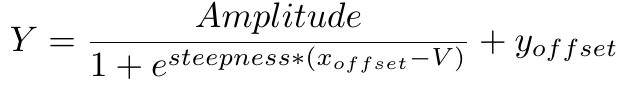
\includegraphics[width=.45\textwidth]{st1.PNG}
				\caption{The ST curve equation}
				\label{fig:STeqn}
			\end{figure}
		We are able to find the parameters for the ST equation under two assumptions. First, under the operating voltage of [-.01,-.1] mV, the contractile tension grows from 0\% to 99\% of the maximum tension. Second, that the ST curve should be centered at -50 mV. Based on these assumptions, the steepness and y-offset of the curve can be determined:
		\begin{align*}
			Y(V) &= \frac{F_{max}}{1+e^{steepness*(x_{offset}-V)}}+y_{offset} \\
			 .99F_{max} &= \frac{F_{max}}{1+e^{-.04S}}+y_{offset} \\
			 0 &= \frac{F_{max}}{1+e^{.05S}}+y_{offset} \\
			 .99F_{max} &= \frac{F_{max}}{1+e^{-.04S}} - \frac{F_{max}}{1+e^{.05S}} \\
			 .99 &= \frac{1}{1+e^{-.04S}} - \frac{1}{1+e^{.05S}} \\
			 S &= 121.465 \\
			 \\
			 .99F_{max} &= \frac{F_{max}}{1+e^{-4.858}}+y_{offset} \\
			 y_{offset} &= F_{max}\bigg(\frac{1}{1+e^{-4.858}}-.99\bigg) \\
			 y_{offset} &= .002294 F_{max}
		\end{align*}
	\section{Muscle Moment Arms}
	Calculating muscle moment arms over the walking cycle is critical to determining joint torques. In order to calculate the total torque on a joint, we must know which muscles contribute to forces about that joint and how long their moment arms are at any given time. Finding a muscle's moment arm boils down to five steps:
		\begin{enumerate}
		  \item Determine which joint to analyze
		  \item Select a muscle to analyze
		  \item Specify a joint axis of interest
		  \item Project the muscle onto the plane specified by that joint axis
		  \item Calculate the distance from the joint axis to the muscle projection
		\end{enumerate}
	I've created a routine to carry out this process using vector geometry. The resulting muscle moment arms can be used to determine when the action of a muscle transitions from flexion to extension and the magnitude of the resulting force. This is a useful tool, as well, because it is able to analyze joints even us they are biarticular. For example, the biceps femoris posterior muscle connects the pelvis and the tibia, spanning the hip and knee joints. This process is capable of analyzing the moment arm profiles for both joints. \par
	Additionally, this program lays the groundwork for analyzing muscle moment arms along axes besides the extensor/flexor axes. As we receive 3D motion for the rat hindlimb, this will become an important tool for determining moment arms along the external/internal rotation and abduction/adduction axes.
		\begin{figure}
			\centering
			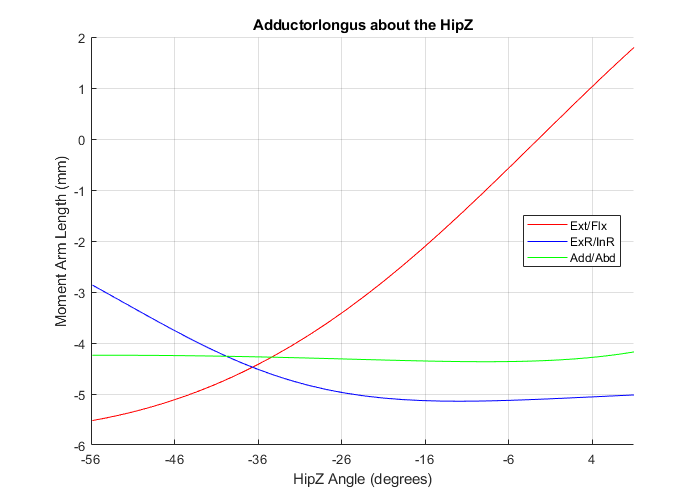
\includegraphics[width=.7\textwidth]{mom1.png}
			\caption{An example schematic of the moment arm profiles of the adductor longus about the hip}
			\label{fig:mom1}
		\end{figure}
		\begin{figure}
			\centering
			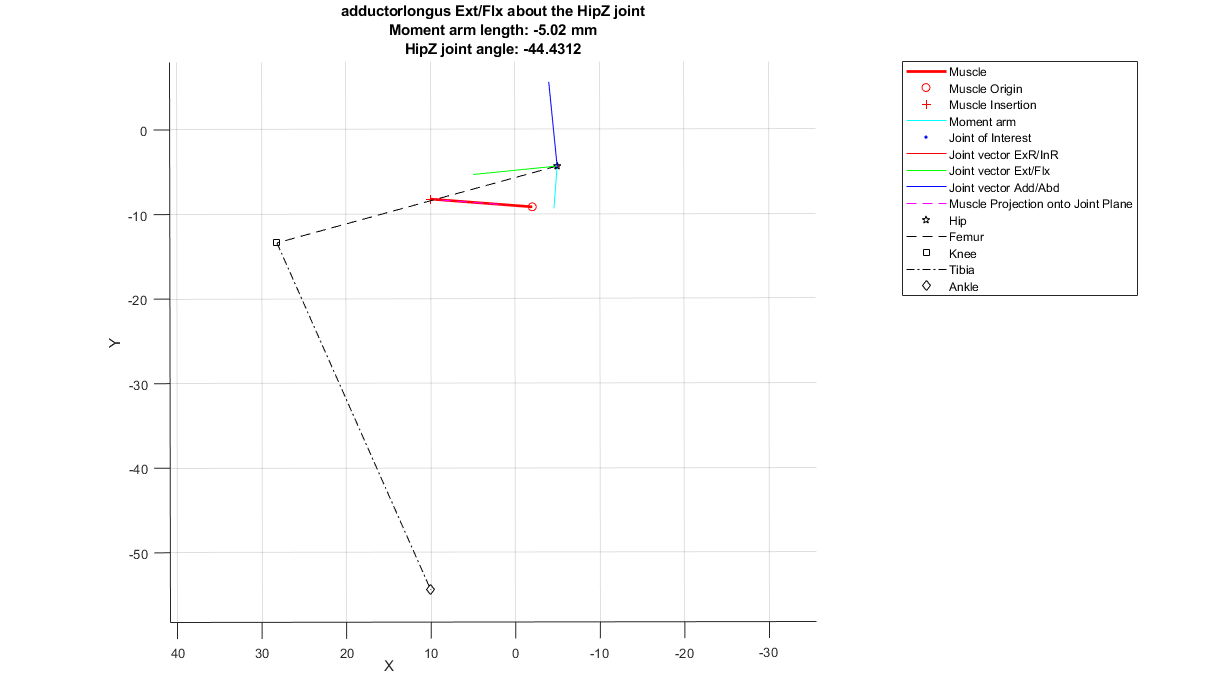
\includegraphics[width=.7\textwidth]{mom2.png}
			\caption{A 3D graphical representation of the moment arm over time to verify the program is working}
			\label{fig:mom2}
		\end{figure}
		\FloatBarrier
	\section{Torque Simulations}
	It's important to note that I've inherited quite a bit of this work from the previous PhD student on the project, Alex Hunt. Alex did a great amount of work in processing the experimental data from Jena and translating that into usable data for the Matlab code he prepared. One important aspect of that code was the generation of a torque profile for the stance and swing phases of gait. \par
	Stance-phase mean joint torque was calculated by our German collaborators for various grades of incline. Data from flat walking was formatted into Nm profiles. A Simulink model of the hind limb was then moved through the kinematic profile to determine the torque about the joints during the swing phase.
		\begin{figure}
			\centering
			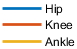
\includegraphics[width=.1\textwidth]{akin4.PNG} \\
			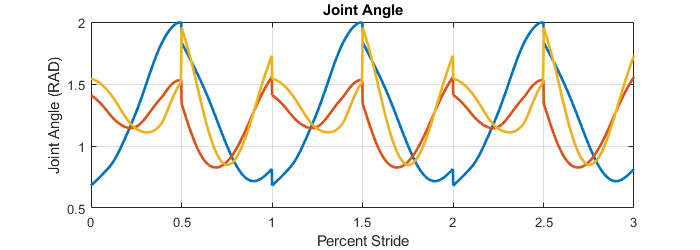
\includegraphics[width=.7\textwidth]{akin1.png} \\
			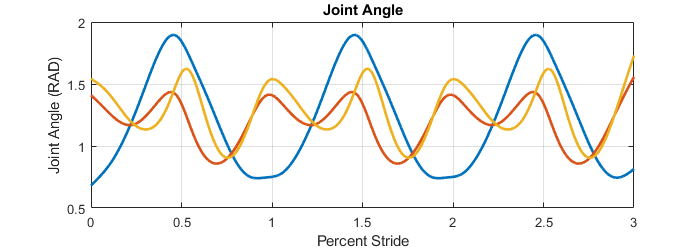
\includegraphics[width=.7\textwidth]{akin2.png} \\
			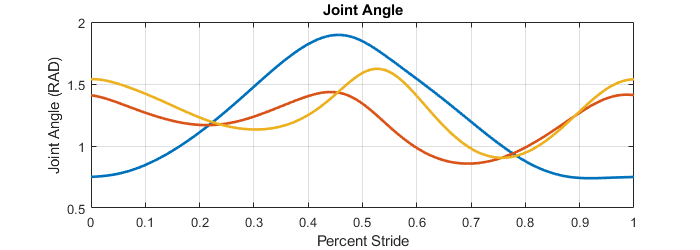
\includegraphics[width=.7\textwidth]{akin3.png}
			\caption{The kinematic profile was data driven in stance, simulated in swing, and then the data was smoothed to create a joint angle profile}
			\label{fig:alexkinematics}
		\end{figure}
		In a similar vein, Alex used torque data from the stance phase of walking and simulated the swing phase, smoothing the resulting signal to generate a complete gait profile.
			\begin{figure}
				\centering
				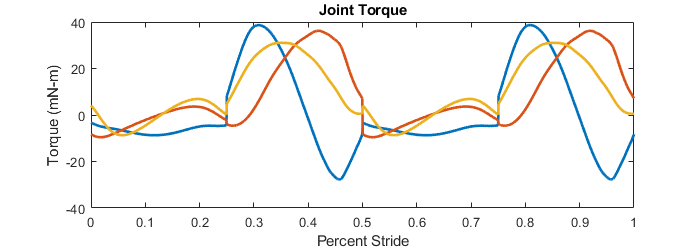
\includegraphics[width=.7\textwidth]{atorque1.png}
				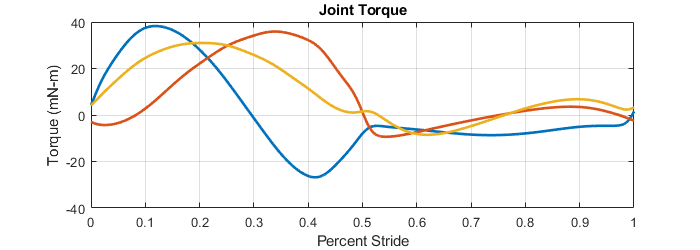
\includegraphics[width=.7\textwidth]{atorque2.png}
				\caption{The torque profile was data driven in stance, simulated in swing, and then the data was smoothed to create a joint angle profile}
				\label{fig:alextorques}
			\end{figure}
	\section{Passive Joint Torque}
	Passive joint torque refers  to the torque generated by the passive properties of the muscles connected to it. As the leg is moved through the stepping cycle, the passive torques will change as the muscle lengths change. In experimental results, passive muscle tension only manifests as the muscle is extended beyond the resting length and is relatively small for the length tension curve as defined above. \par
		\begin{figure}
			\centering
			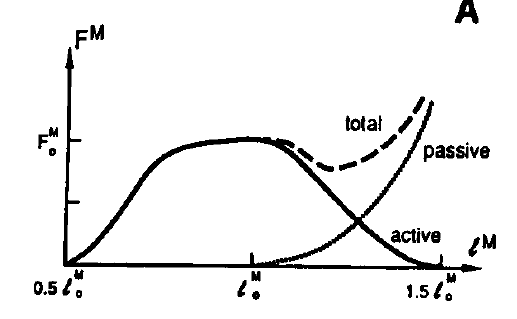
\includegraphics[width=.7\textwidth]{lwidth3.PNG}
			\caption{Nominal length-tension curve for muscle}
			\label{fig:passX}
		\end{figure}
	Computing the passive joint torque involves determining which muscles to analyze and calculating their passive tension over a walking cycle. This tension, coupled with the simulated muscle moment arms discussed previously, allow us to calculate the passive torque contributions of every muscle. Passive muscles tension is calculated using a discretized version of the Hill passive tension equation.
		\begin{align*}
			\frac{dT}{dt} &= \frac{K_{se}}{c}\bigg[K_{pe}(L-L_{rest})+c \dot{L}-\big(1+\frac{K_{pe}}{K_{se}}\big)\bigg] \\
			\frac{T_{i}-T_{i-1}}{dt} &= \frac{K_{se}}{c}\bigg[K_{pe}(L_{i}-L_{rest})+c \dot{L_{i}}-\big(1+\frac{K_{pe}}{K_{se}}\big)\bigg] \\
			P &= \frac{K_{se} dt}{c} \\
			T_{i}-T_{i-1} &= P K_{pe}x+Pc\dot{x} -P\big(1+\frac{K_{pe}}{K_{se}}\big)T_{i} \\
			T_{i}\big[1+P\big(1+\frac{K_{pe}}{K_{se}}\big)\big] &= P K_{pe}x+Pc\dot{x}+T_{i-1}\\
			T_{i} &= \frac{P K_{pe}x+Pc\dot{x}+T_{i-1}}{1+P\big(1+\frac{K_{pe}}{K_{se}}\big)} \\
			&= \frac{K_{pe}x+c\dot{x}+\frac{1}{P}T_{i-1}}{\frac{1}{P}+\big(1+\frac{K_{pe}}{K_{se}}\big)} \\
			&= \frac{K_{pe}(L_i-L_{min})+c\dot{L}+\frac{c}{K_{se}dt}T_{i-1}}{1+\frac{K_{pe}+\frac{c}{dt}}{K_{se}}}
		\end{align*}
	where the resting length is set to $L_{min}$, $c$ is the muscle damping constant, and $dt$ is the simulation timestep which, in this case, is 5E-4s. The tension profile is initialized such that $T_{0} = 0$. By iterating this function from $L_{min}$ to $L_{max}$ over the course of a step cycle, it is possible to produce a length tension reference curve that is then used to calculate joint passive torque. With the leg in a certain configuration, the muscle lengths are calculated, the passive tension is determined for that length, and is then multiplied by the instantaneous moment arm. Summing these passive torques for all relevant muscles results in continuous passive joint torque, as seen in Fig. \ref{fig:pass1}.
		\begin{figure}
			\centering
			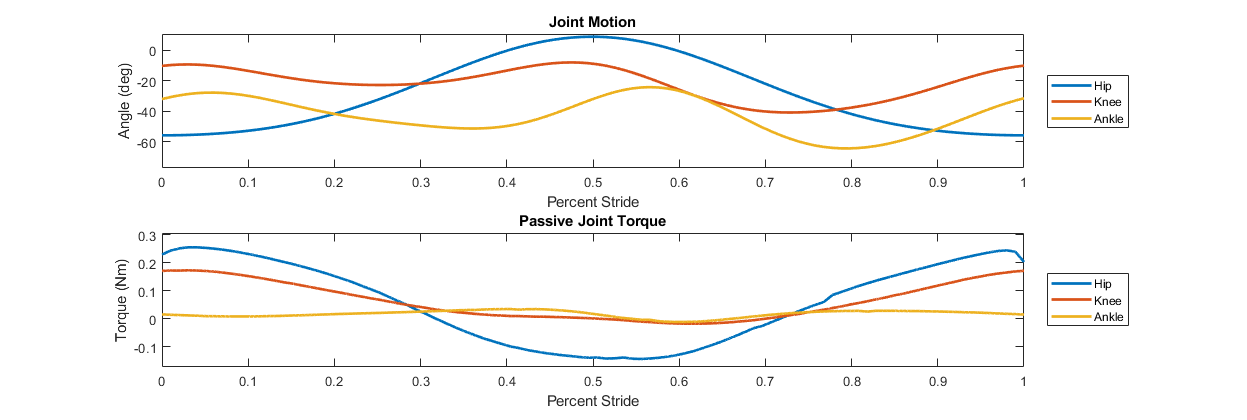
\includegraphics[width=.8\textwidth]{pass1.png}
			\caption{The passive joint torque and associated joint motion}
			\label{fig:pass1}
		\end{figure}
	\section{Load Torque}
	The second type of torque that must be calculated for the model is the load torque caused by the weight of the animal pushing on the ground. A small sampling of toe point load forces were calculated by our colleagues in Jena and can be used to determine joint torque. This data set includes sagittal plane forces in the x- and y-directions during four distinct phases of the step cycle: toe contact, mid-stance, toe off, and mid-swing. \par
	Forces at an end effector can elicit torques in the joints of multi-link arms. Referring to Murray, Li, and Sastry's 1994 book \underline{A Mathematical Introduction to Robotic Manipulation}\cite{murray_mathematical_1994}, joint torques can be calculated by first calculating the spatial manipulator Jacobian. The spatial manipulator Jacobian is an operator that represents the relationship between joint positions and joint axes, allowing a user to multiply force vectors and output joint torques. The composition of the spatial manipulator jacobian is a 6$\times$n matrix of the form:
	\begin{align*}
		J^{s}_{st} =
		\begin{bmatrix}
			-\omega_{n} \times q_n \\
			\omega_{n}
		\end{bmatrix}
	\end{align*}
	where $\omega$ represents the joint axis and $q_{n}$ represents a joint's global coordinates. For example, at a leg configuration of $[-54.1^{\circ}, -11.0^{\circ},-28.4^{\circ}]$,
	\begin{align*}
		q_{H} &= \begin{bmatrix}
			-4.99 \\
			-4.35 \\
			10.36
			\end{bmatrix}
		q_{K} = \begin{bmatrix}
			29.23 \\
			-7.78 \\
			20.13
			\end{bmatrix}
		q_{A} = \begin{bmatrix}
			25.69 \\
			-52.55 \\
			20.33
			\end{bmatrix} \\
		\omega_{H} &= \begin{bmatrix}
			-0.059 \\
			-0.007 \\
			-0.998
			\end{bmatrix}
		\omega_{K} = \begin{bmatrix}
			0.059 \\
			0.006 \\
			0.998
			\end{bmatrix}
		\omega_{A} = \begin{bmatrix}
			-0.059 \\
			-0.007 \\
			-0.998
			\end{bmatrix}
	\end{align*}
	where the $q$ vectors represent the global joint positions and the $\omega$ vectors represent the joint axes of the hip, knee, and ankle. Values above are shown in millimeters for clarity but are processed in meters when computing the jacobian. The $\omega$ terms above represent the sagittal motion joint axes in global coordinates, as well. The resulting spatial manipulator jacobian takes the form of:
		\begin{align*}
			J^{s}_{st} &= 
				\begin{bmatrix}
				    0.0044  & -0.0079  &  0.0526 \\
				   -0.0056  & -0.0280  &  0.0244 \\
				   -0.0002  &  0.0006  & -0.0033 \\
				   -0.0594  &  0.0594  & -0.0594 \\
				   -0.0072  &  0.0064  & -0.0068 \\
				   -0.9982  &  0.9982  & -0.9982
				\end{bmatrix}
		\end{align*}
	For the current model, I'm using ground reaction forces calculated by Gillian Muir's 1999 paper "Ground reaction forces in locomoting hemi-parkinsonian rats: a definitive test for impairments and compensations"\cite{muir_ground_1999}. The data, shown in Fig. \ref{fig:grfdata} used is for the control rat and I isolated only the hindlimb contact portion. Since ground reaction forces only induce joint torque when the hindlimb is in contact with the ground, all swing phase forces are set to zero. With Alex's normalized walking pattern, that means that ground reaction forces can be set to zero for the second half of stride. In an effort to make the signal continuous, I connected three steps together and then smoothed the data to fit.
		\begin{figure}
			\centering
			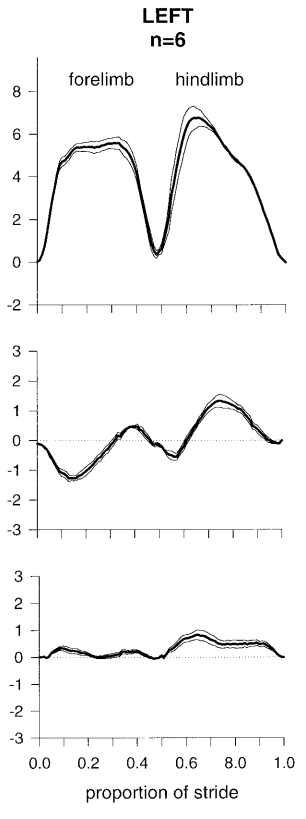
\includegraphics[width=.3\textwidth]{loadt3.PNG}
			\caption{The ground reaction forces for a rat}
			\label{fig:grfdata}
		\end{figure}
	Using the ground reaction force data and the spatial manipulator jacboian, we can calculate the load torque in all three joints in the sagittal plane. By constructing a wrench at the toe position,
		\begin{align*}
			F &= 
				\begin{bmatrix}
					F_{x} \\
					F_{y} \\
					F_{z} \\
					0 \\
					0 \\
					0
				\end{bmatrix}
		\end{align*}
	load joint torques can be calculated as
	\begin{align*}
		\tau &= (J^{s}_{st})^{T}F_{s}
	\end{align*}
	Using this information, the resulting load torque profile looks like
		\begin{figure}
			\centering
			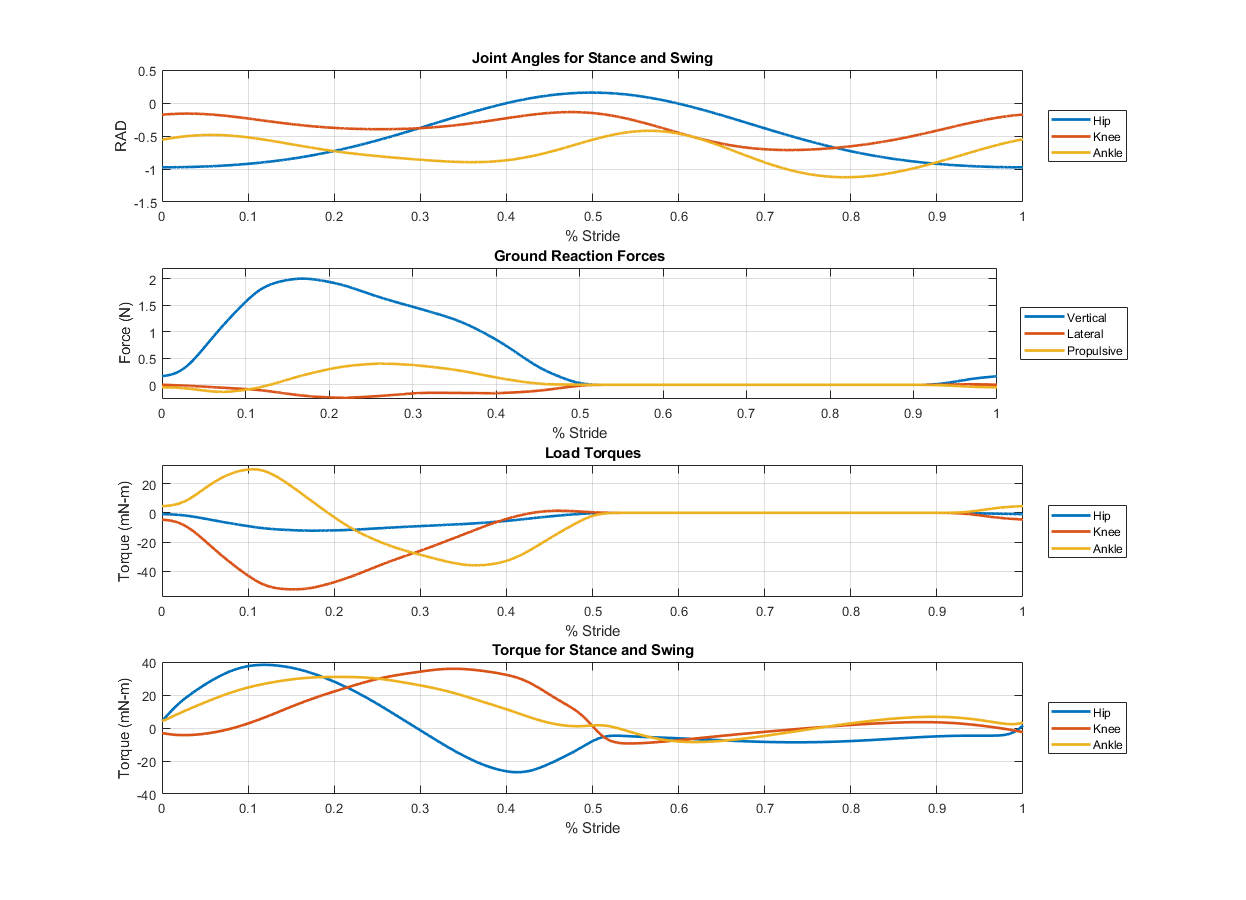
\includegraphics[width=\textwidth]{loadt1.png}
			\caption{Ground reaction forces, load torques, and the total leg torque from data}
			\label{fig:loadt1}
		\end{figure}
	
	\section{Total Passive Load Torque}
		The total passive joint torque is the combination of the muscle passive torque and the load torque. The resulting torque profile is shown in Fig. \ref{fig:loadt2}. Ultimately the load joint torque contributes much less to the overall passive torque profile than the passive muscle torque profile. The impact of its inclusion can be seen in the total joint torque profile where the shaded region represents the deviation of the total torque profile from the passive muscle joint torque
		\begin{figure}
			\centering
			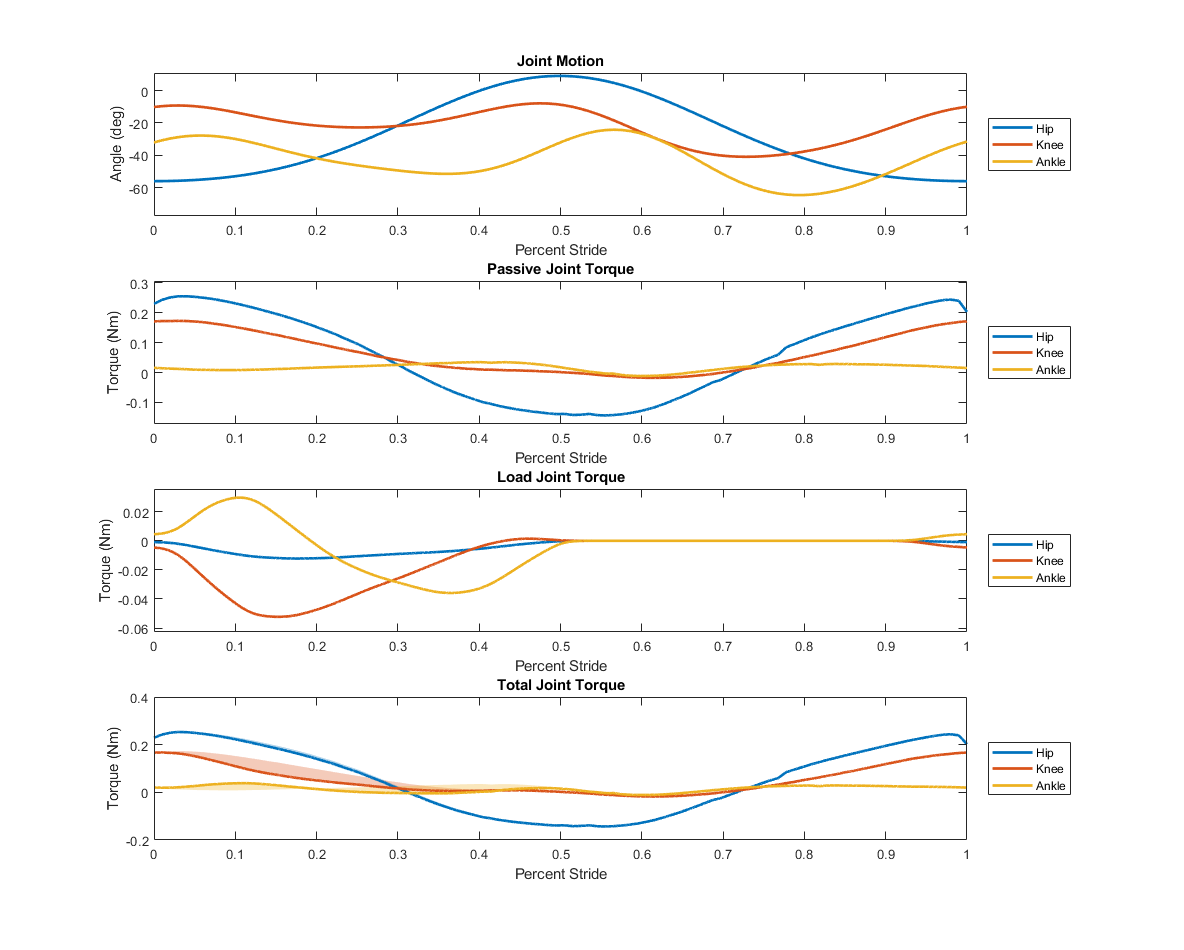
\includegraphics[width=\textwidth]{loadt2.png}
			\caption{Ground reaction forces, load torques, and the total leg torque from data}
			\label{fig:loadt2}
		\end{figure}
		\\
		First, muscle attachment points, $\bar{p}_{att,i}$, are projected onto the plane of interest defined by the joint axis $\bar{j}$. Muscle segments are represented by the subtraction of projection attachment positions.
				\begin{align*}
					\vec{p}_{proj,i} &= \frac{\bar{p}_{att,i} \cdot \vec{j}}{||\bar{j}||^2}\bar{j} \\
					\vv{p}_{i} &= \bar{p}_{proj,i+1}-\bar{p}_{proj,i}
				\end{align*}
		The projected muscle segment is then crossed with the joint axis to determine the moment arm's direction. The moment arm, represented by $\bar{r}_{i}$, is then scaled such that it intersects the muscle projection. 
				\begin{align}
					\bar{r}_{i} &= \bar{p}_{i} \times \bar{j}
				\end{align}
		Finally, the sign of the moment arm, $s_{i}$, is calculated by taking the cross product of the moment arm and the muscle projection then taking the dot product with the joint axis. Positive moment arms induce positive moments, and vice versa. The final moment arm vector is represented as $\bar{r}_{T}$.
		\begin{align}
			s_{i} &= sign\big((\bar{r}_{i} \times \bar{p}_{i}) \cdot \bar{j}\big) \\
			\bar{r}_{T,i} &= s_{i}*\bar{r}_{i}
		\end{align}
		Multi-segment muscles with $n$ number of segments use the previous method to develop amatrix of moment arms, $M^{3 \times n}$. In order to rescale the lengths of the moment arms without losing their planar orientation, we calculate the Euclidean norm of each moment arm and normalize matrix $M$.
		\begin{align}
			||\bar{r}_{i}|| &= \sqrt{\sum_{k=1}^{3}|\bar{r}_{k}|^2}	
		\end{align}
		The proximal projected attachment points for each muscle segment are found relative to the joint center, represented as $\bar{p}_{rel}$. A scaling vector, $\bar{c}$ is calculated by dividing the lengths of all relative attachment distances by the length of the nearest attachments point. This scaling factor is then inverted such that the longer distance a projected relative attachment is from the minimum attachment, the more penalty it incurs. This has the effect of prioritizing the moment arm length of the nearest muscle segment.
		\begin{align}
			\bar{p}_{rel} &= \bar{p}_{proj} - \bar{p}_{joint} \\
			\bar{r}_{rel,i} &= \bar{r}_{i} - \bar{p}_{joint} \\
			||M_{i,:}||_{2} &= \frac{\bar{r}_{rel,i}}{||\bar{r}_{rel,i}||} \\
			c_{i} &= \frac{min(||\bar{p}_{rel}||)}{\bar{p}_{rel,i}}
		\end{align}
		A final scale factor, $t$, was calculated by multiplying the original moment arm lengths with the square of the scale factor. This has the effect of shortening the moment arms from distal segments while maintaining the length of proximal segments.
		\begin{align}
			t_{i} &= \bar{r}_{rel,i}*c_{i}^2
		\end{align}
		This scale factor is then applied back to the normalized moment matrix. A single moment arm is calculated by taking the mean of the scaled planar moment arms. To prioritize the length of the near segment, the maximum scale factor is increased by a factor equal to the number of segments.
		\begin{align}
			\bar{r}_{T} = mean(t*||M|||_{2}) 
		\end{align} 
		\FloatBarrier
		
		\bibliography{ResearchReport1} 
		\bibliographystyle{ieeetr}
		
\end{document}